\chapter{Obrázky}


\begin{figure}[h]
    \centering
    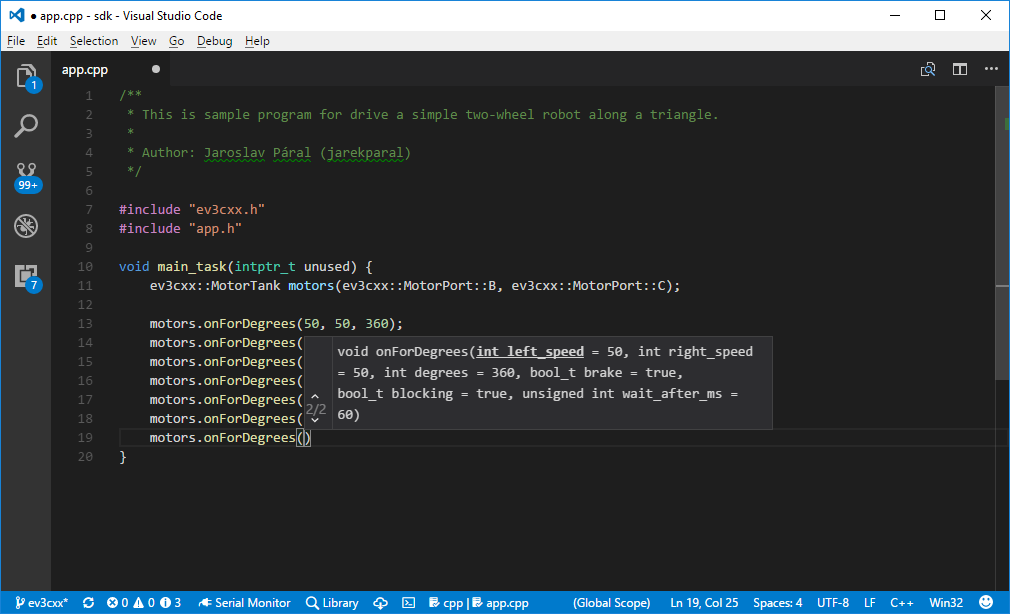
\includegraphics[width=\textwidth]{images/visual-studio-code_intellisense-param.png}
    \caption{Ukázka našeptávání ve Visual Studio Code -- zobrazování parametrů funkce}
    \label{fig:visual-studio-code_intellisense-param}
\end{figure}


\begin{figure}[h]
	\centering
	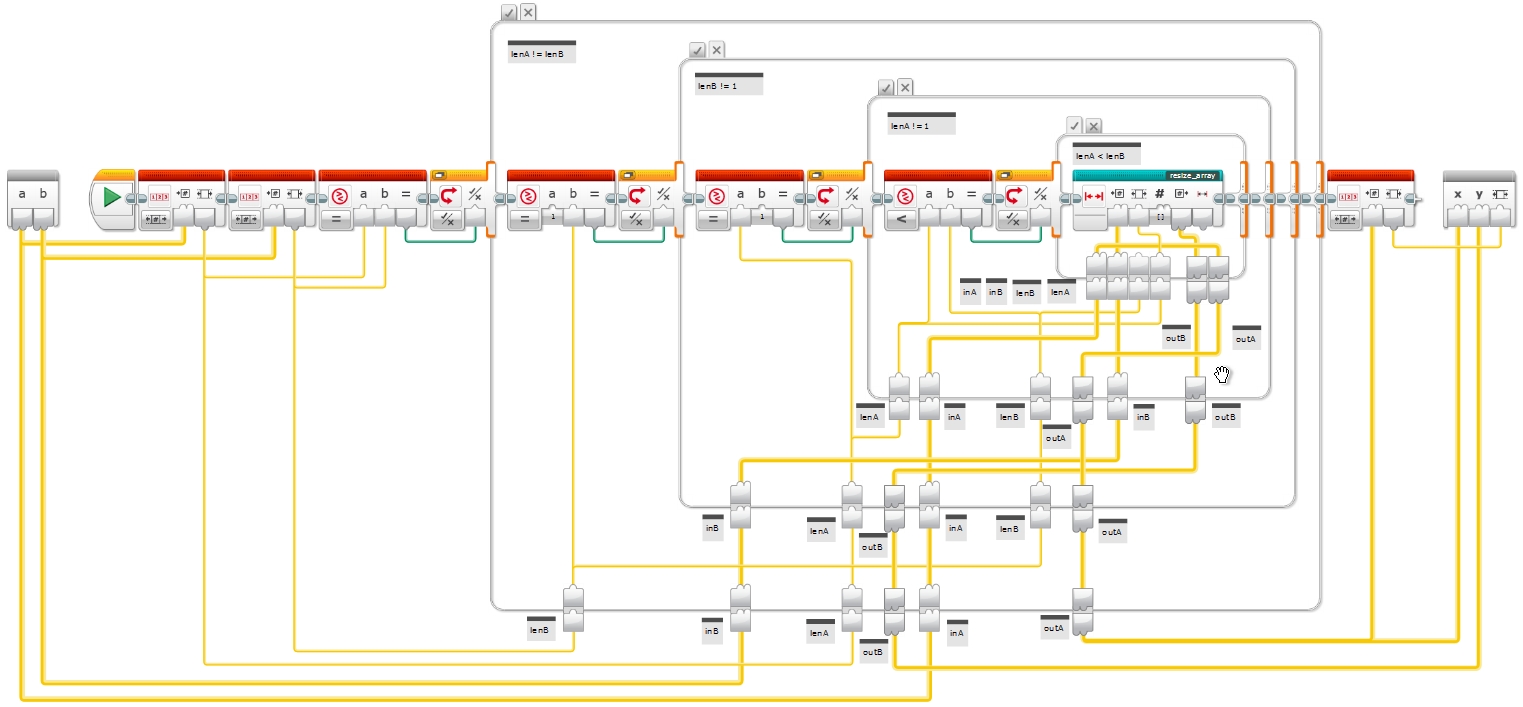
\includegraphics[angle=-90,origin=c,width=280px]{images/lego-soft_legolib_match_array_length.png}
	\caption[Předávání hodnot v~\legoSW{}]{Předávání hodnot v~\legoSW{}}
	\label{fig:lego-soft_legolib_match_array_length}
\end{figure}



\chapter{Ukázka návodu k~C++ API}

Výběr 1 až 3 kapitoly z EV3RT C++ API dokumentace. Kompletní verze k dispozici na \url{http://rb3rt.readthedocs.io/}.

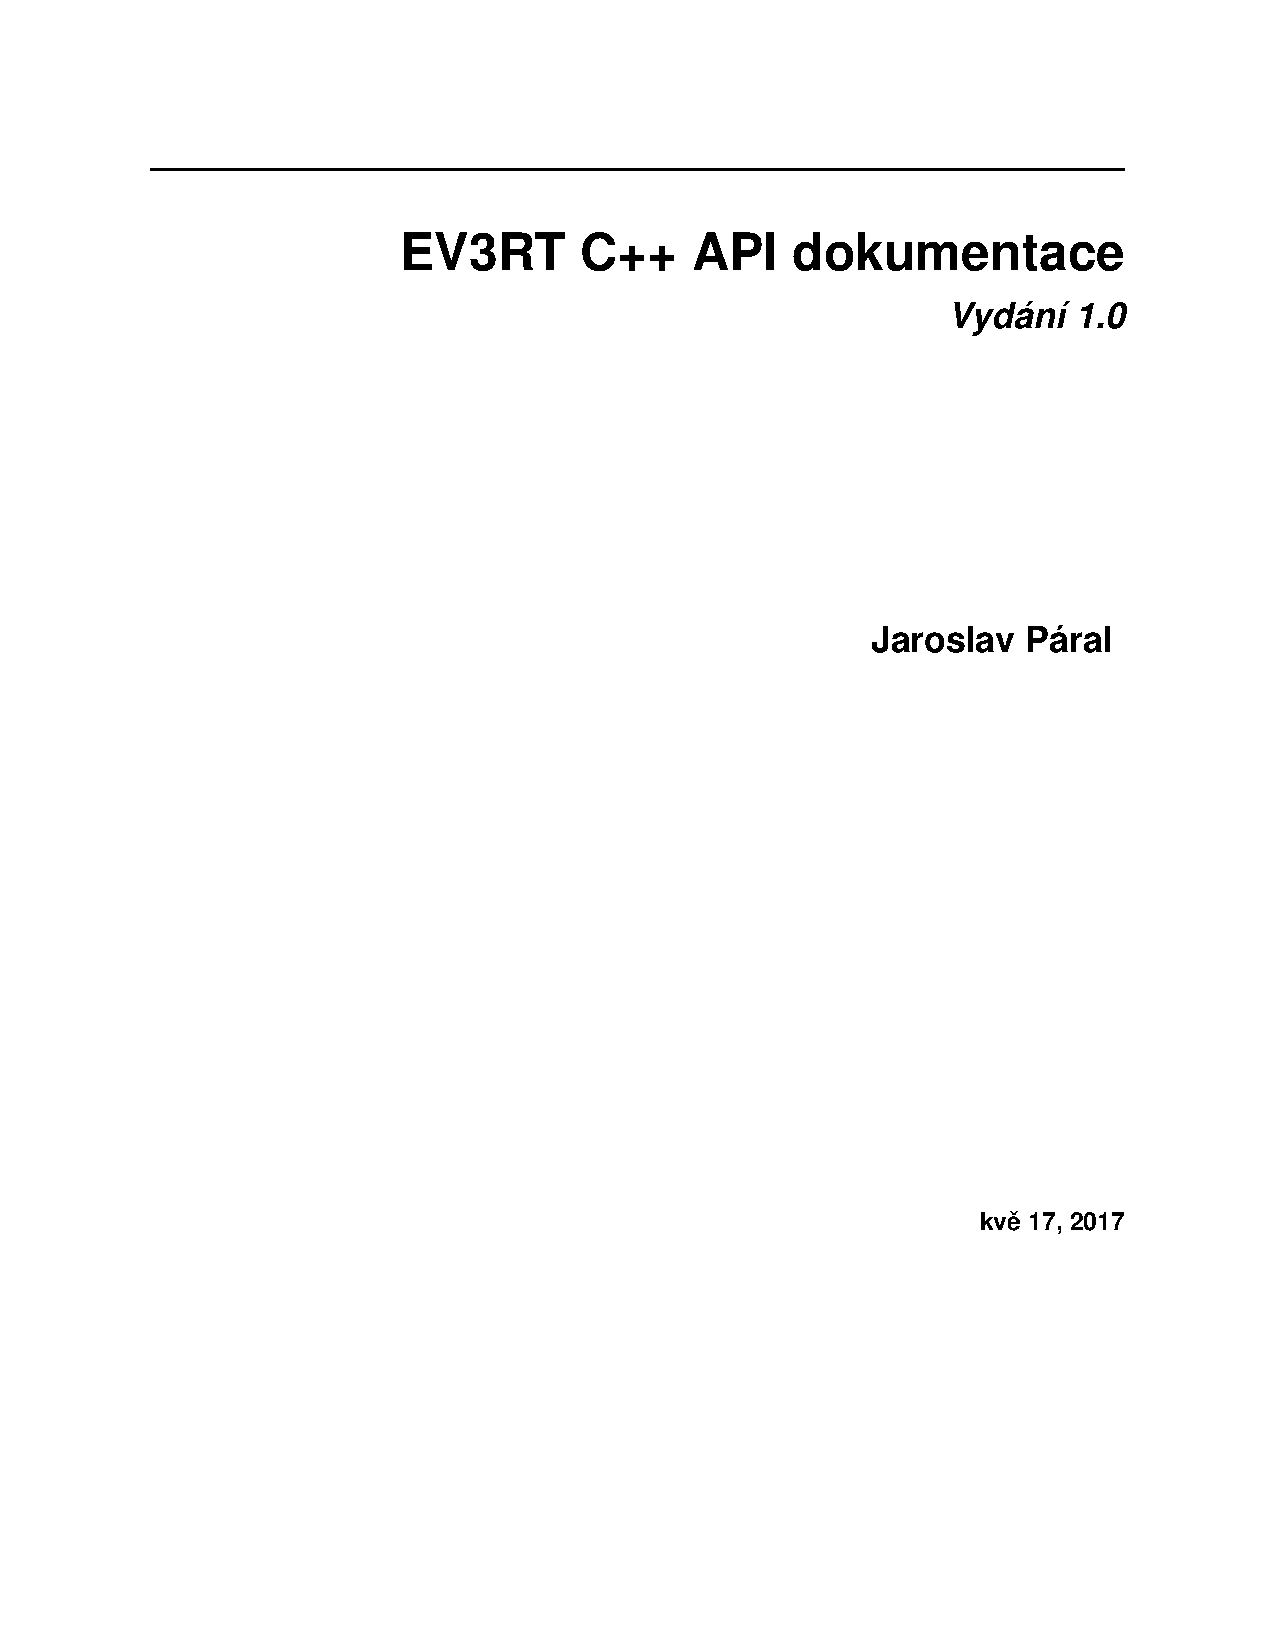
\includepdf[page=7]{ev3rt-cxx-api-doc.pdf}
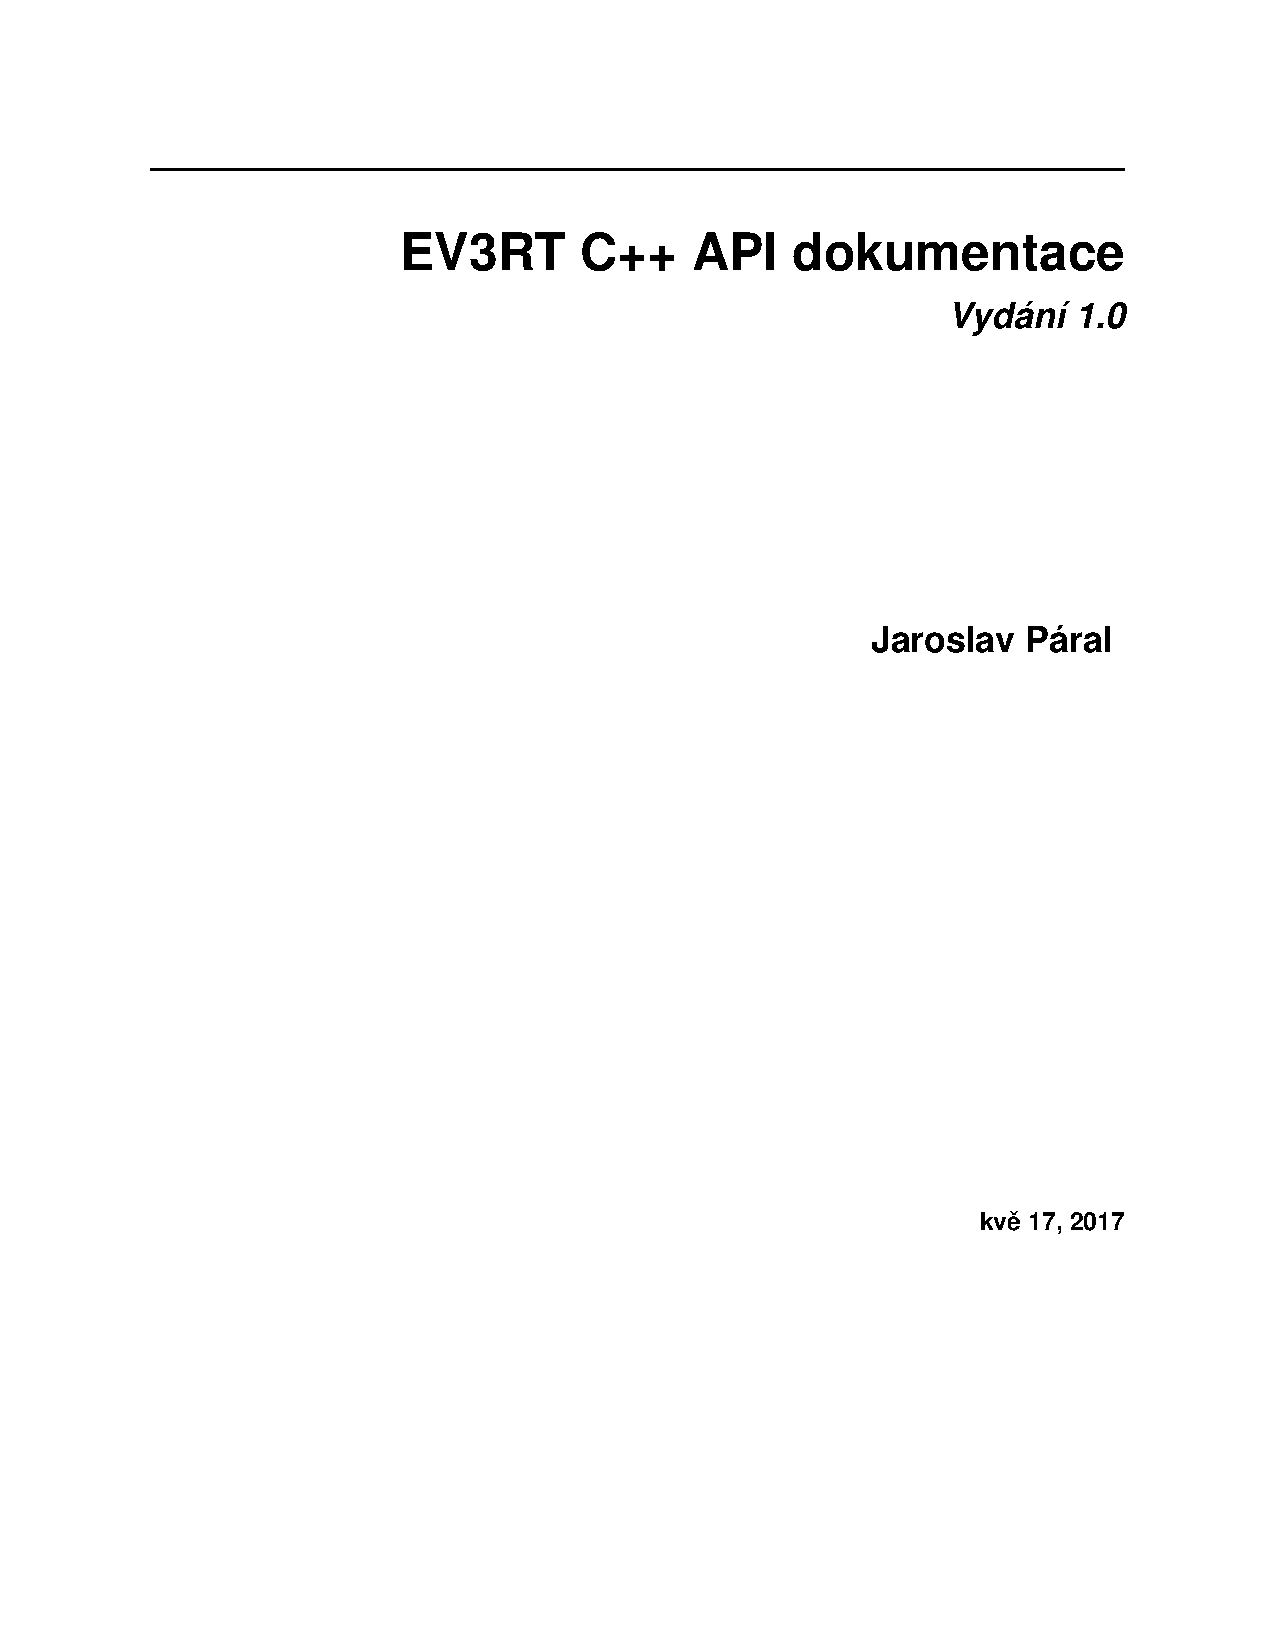
\includepdf[page=8]{ev3rt-cxx-api-doc.pdf}
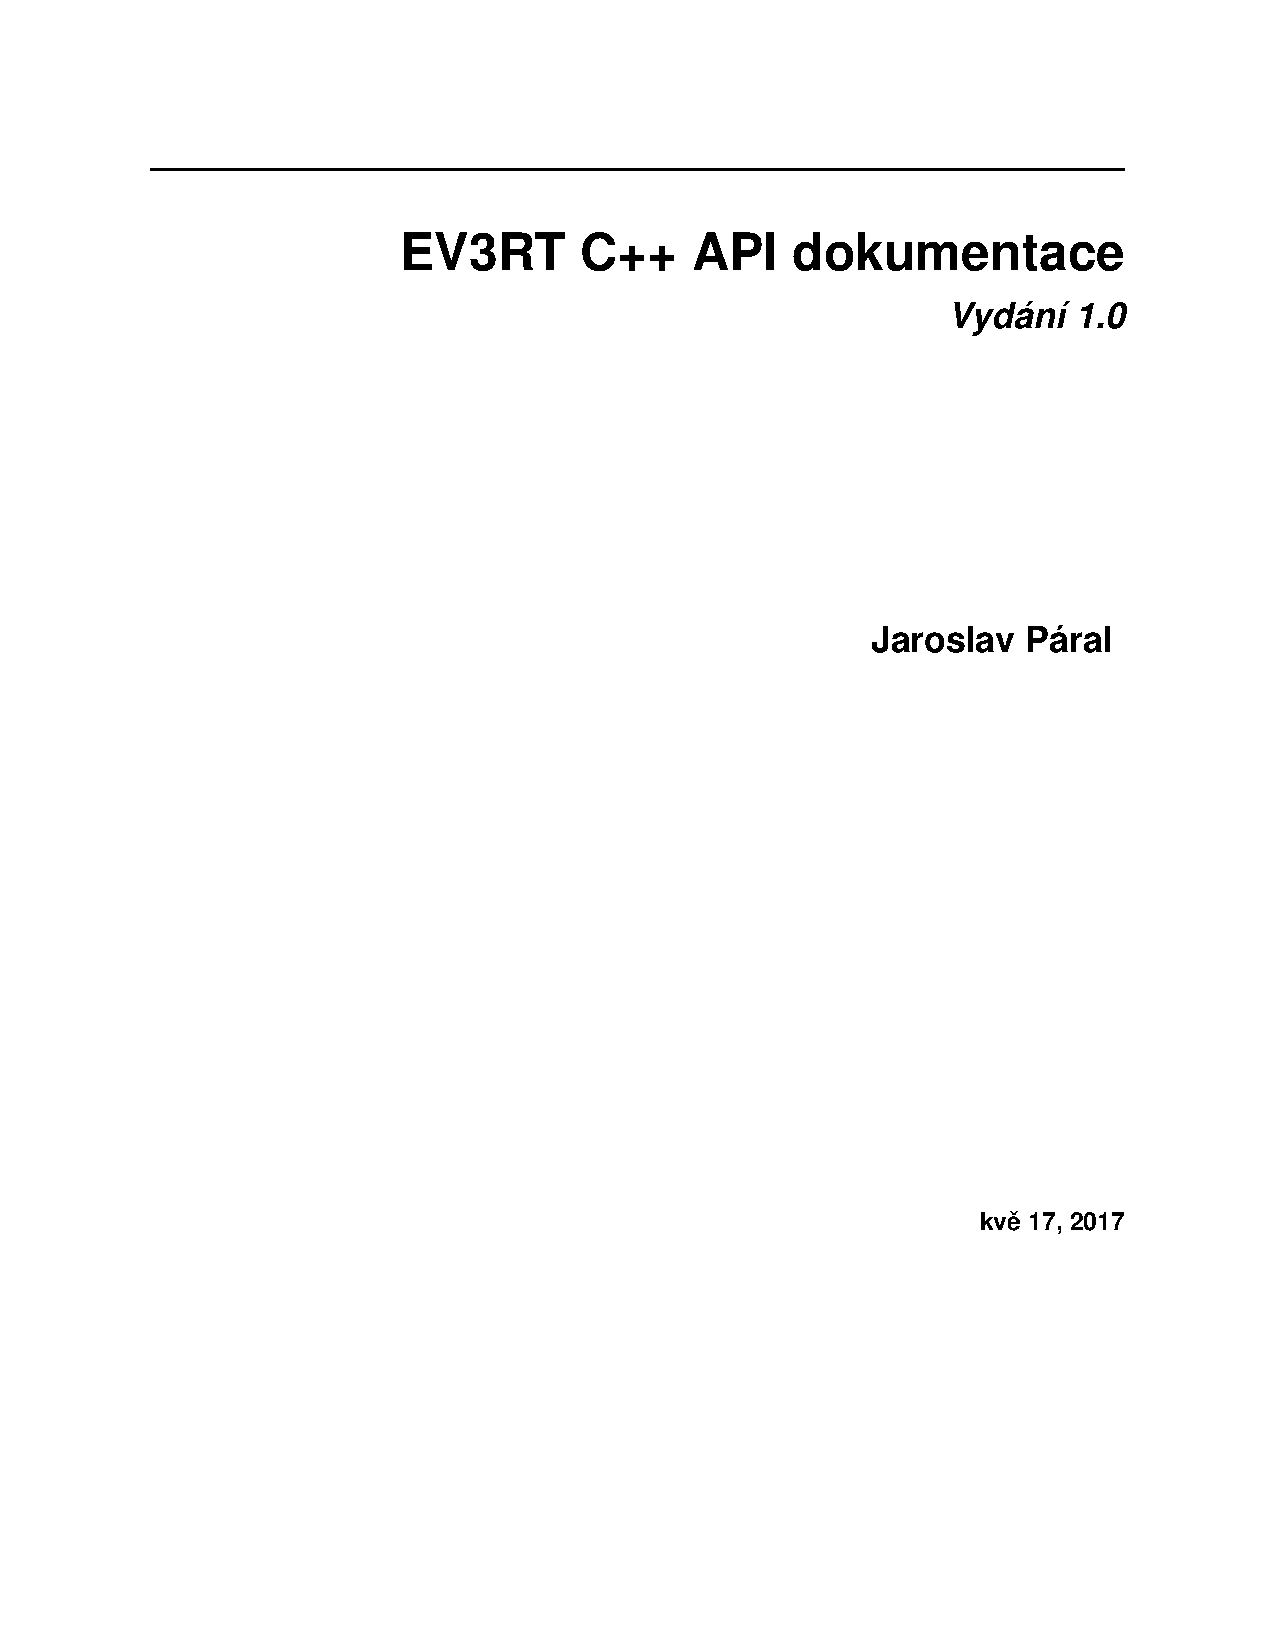
\includepdf[page=9]{ev3rt-cxx-api-doc.pdf}
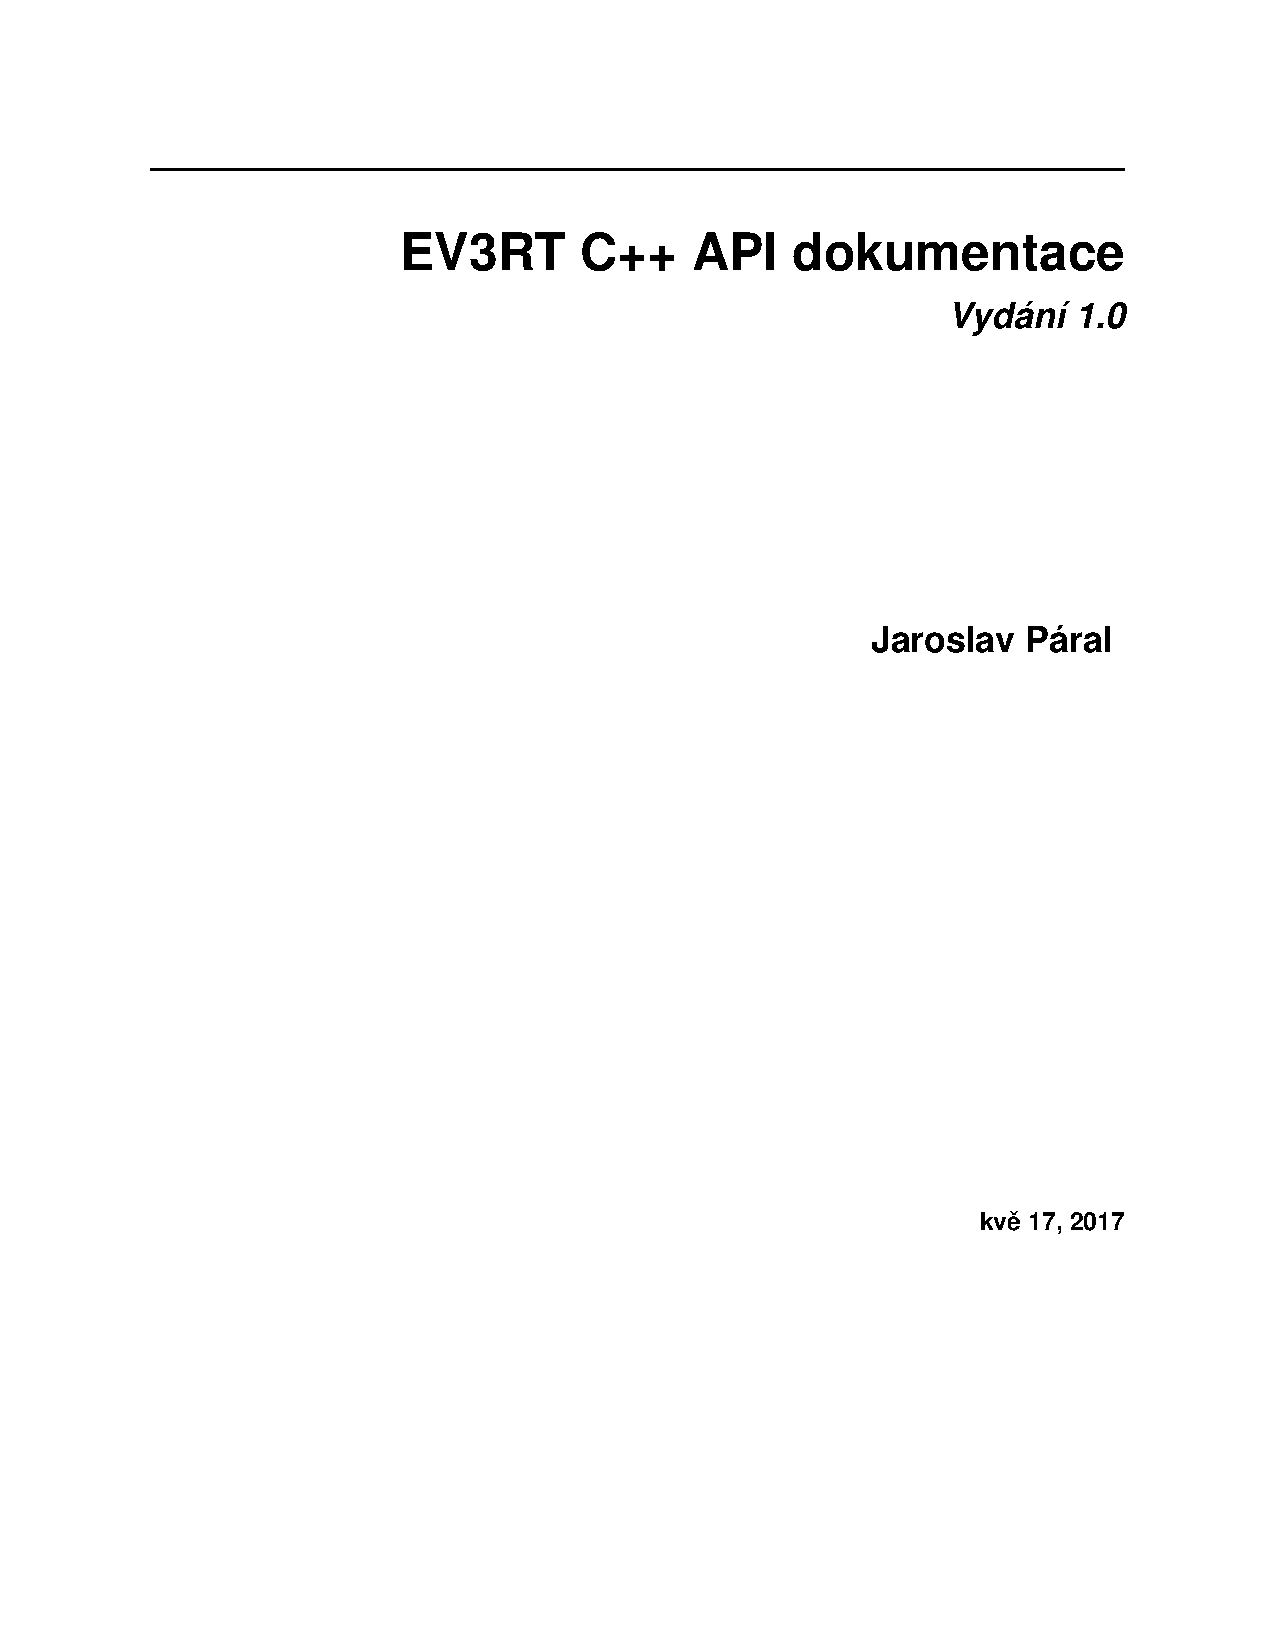
\includepdf[page=10]{ev3rt-cxx-api-doc.pdf}
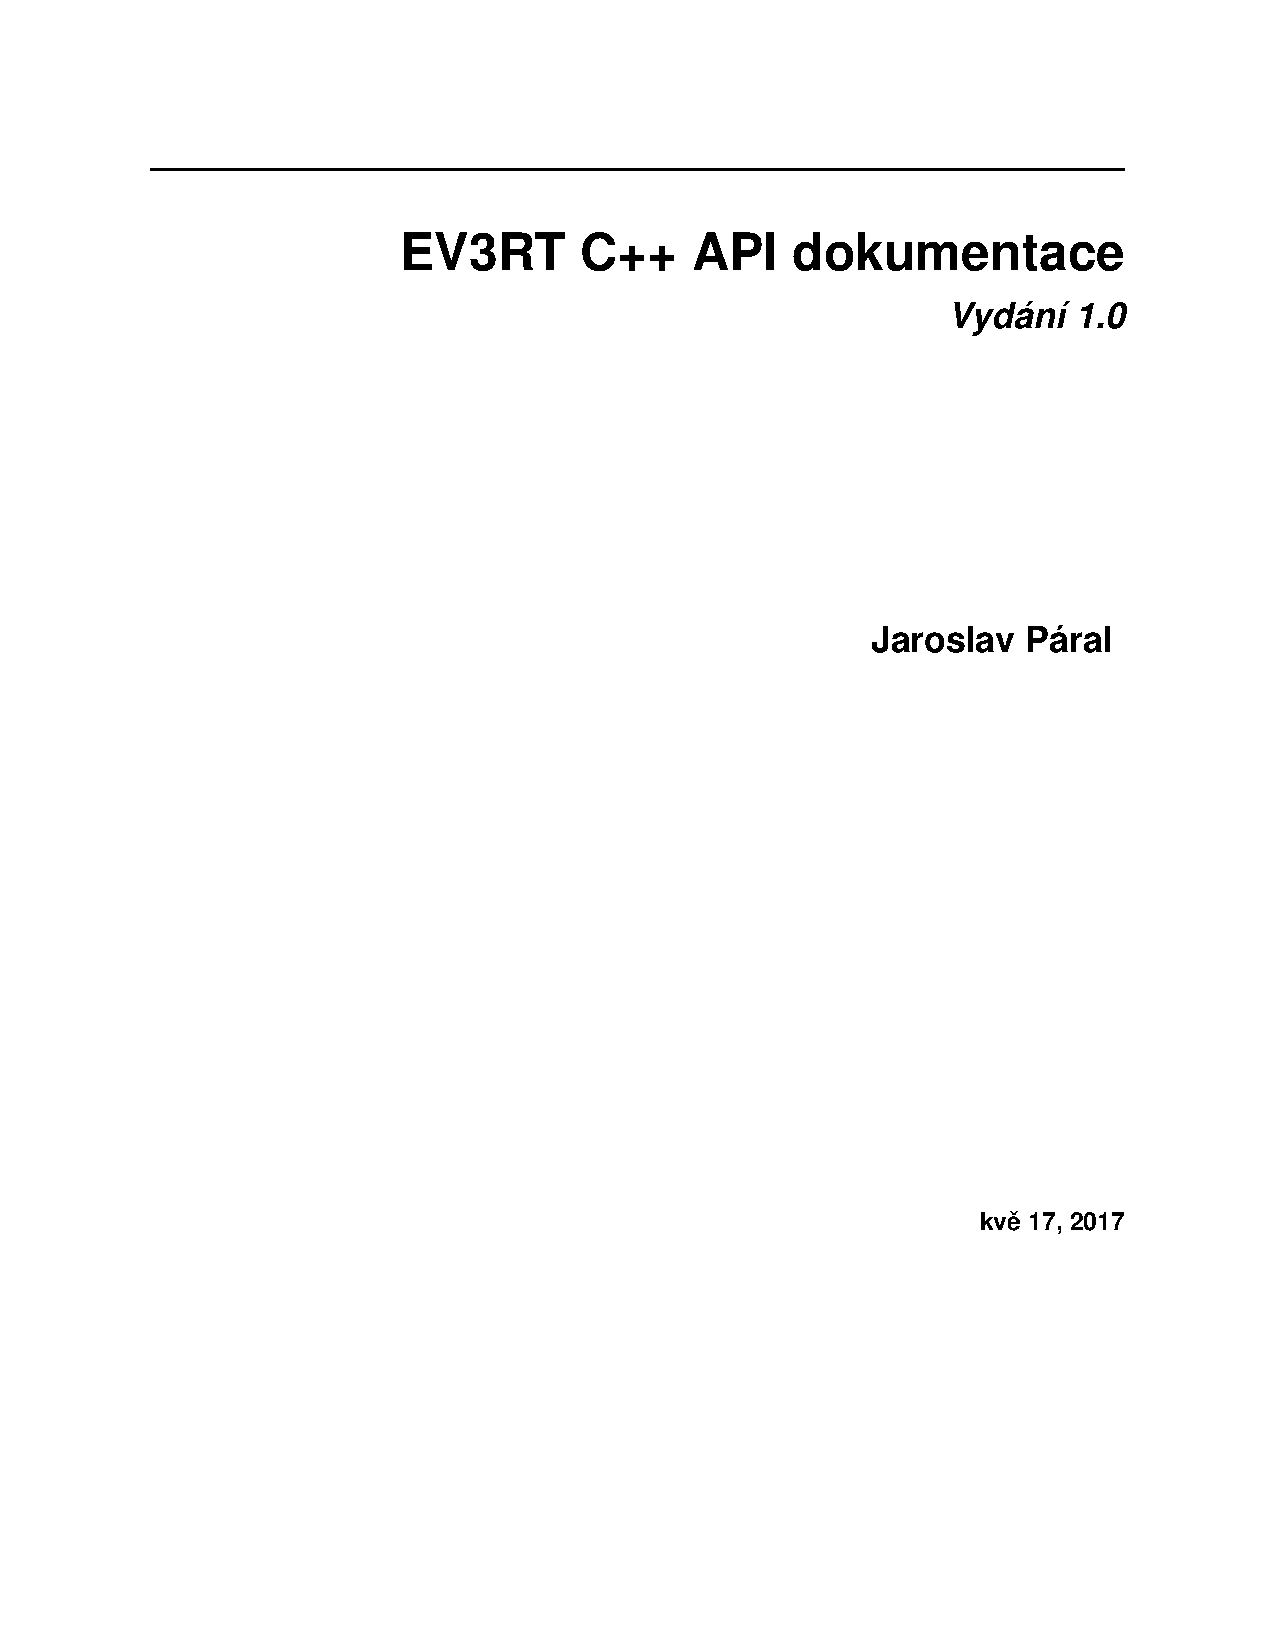
\includepdf[page=11]{ev3rt-cxx-api-doc.pdf}
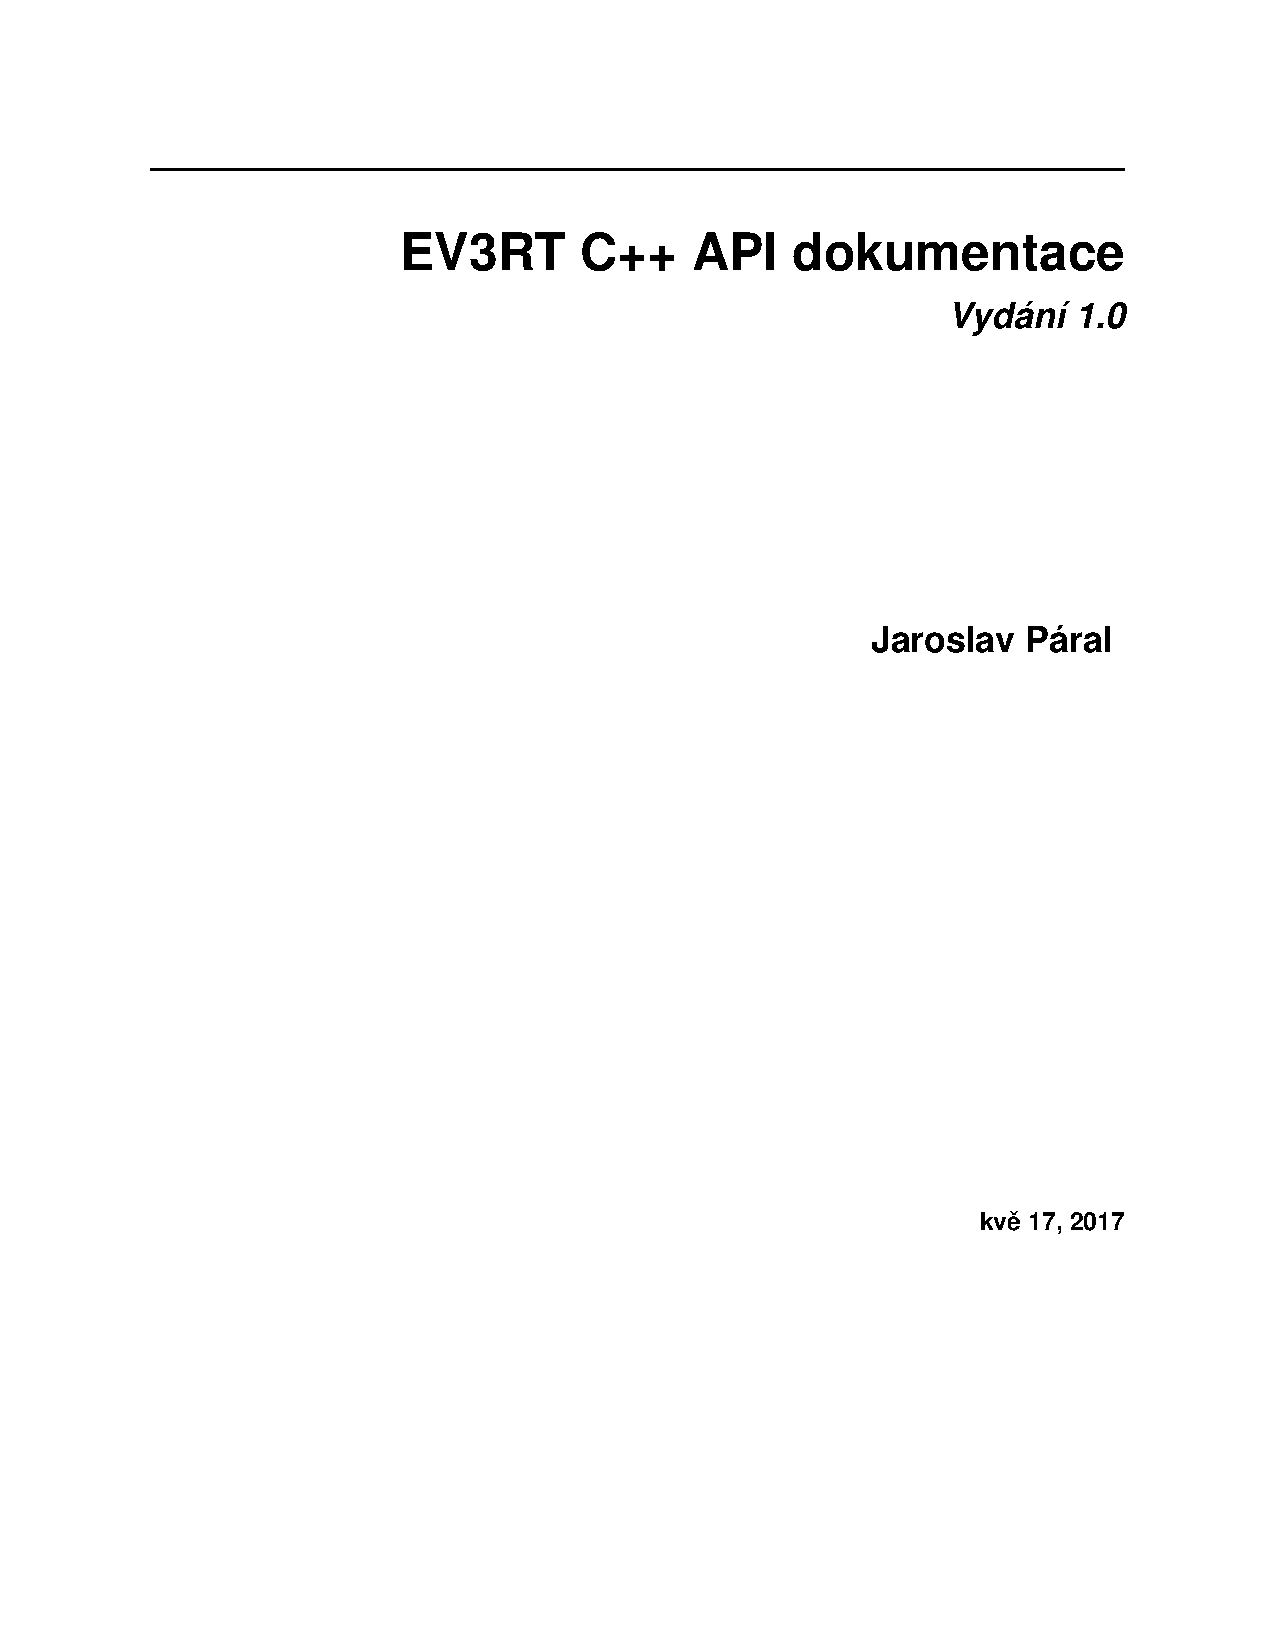
\includepdf[page=12]{ev3rt-cxx-api-doc.pdf}
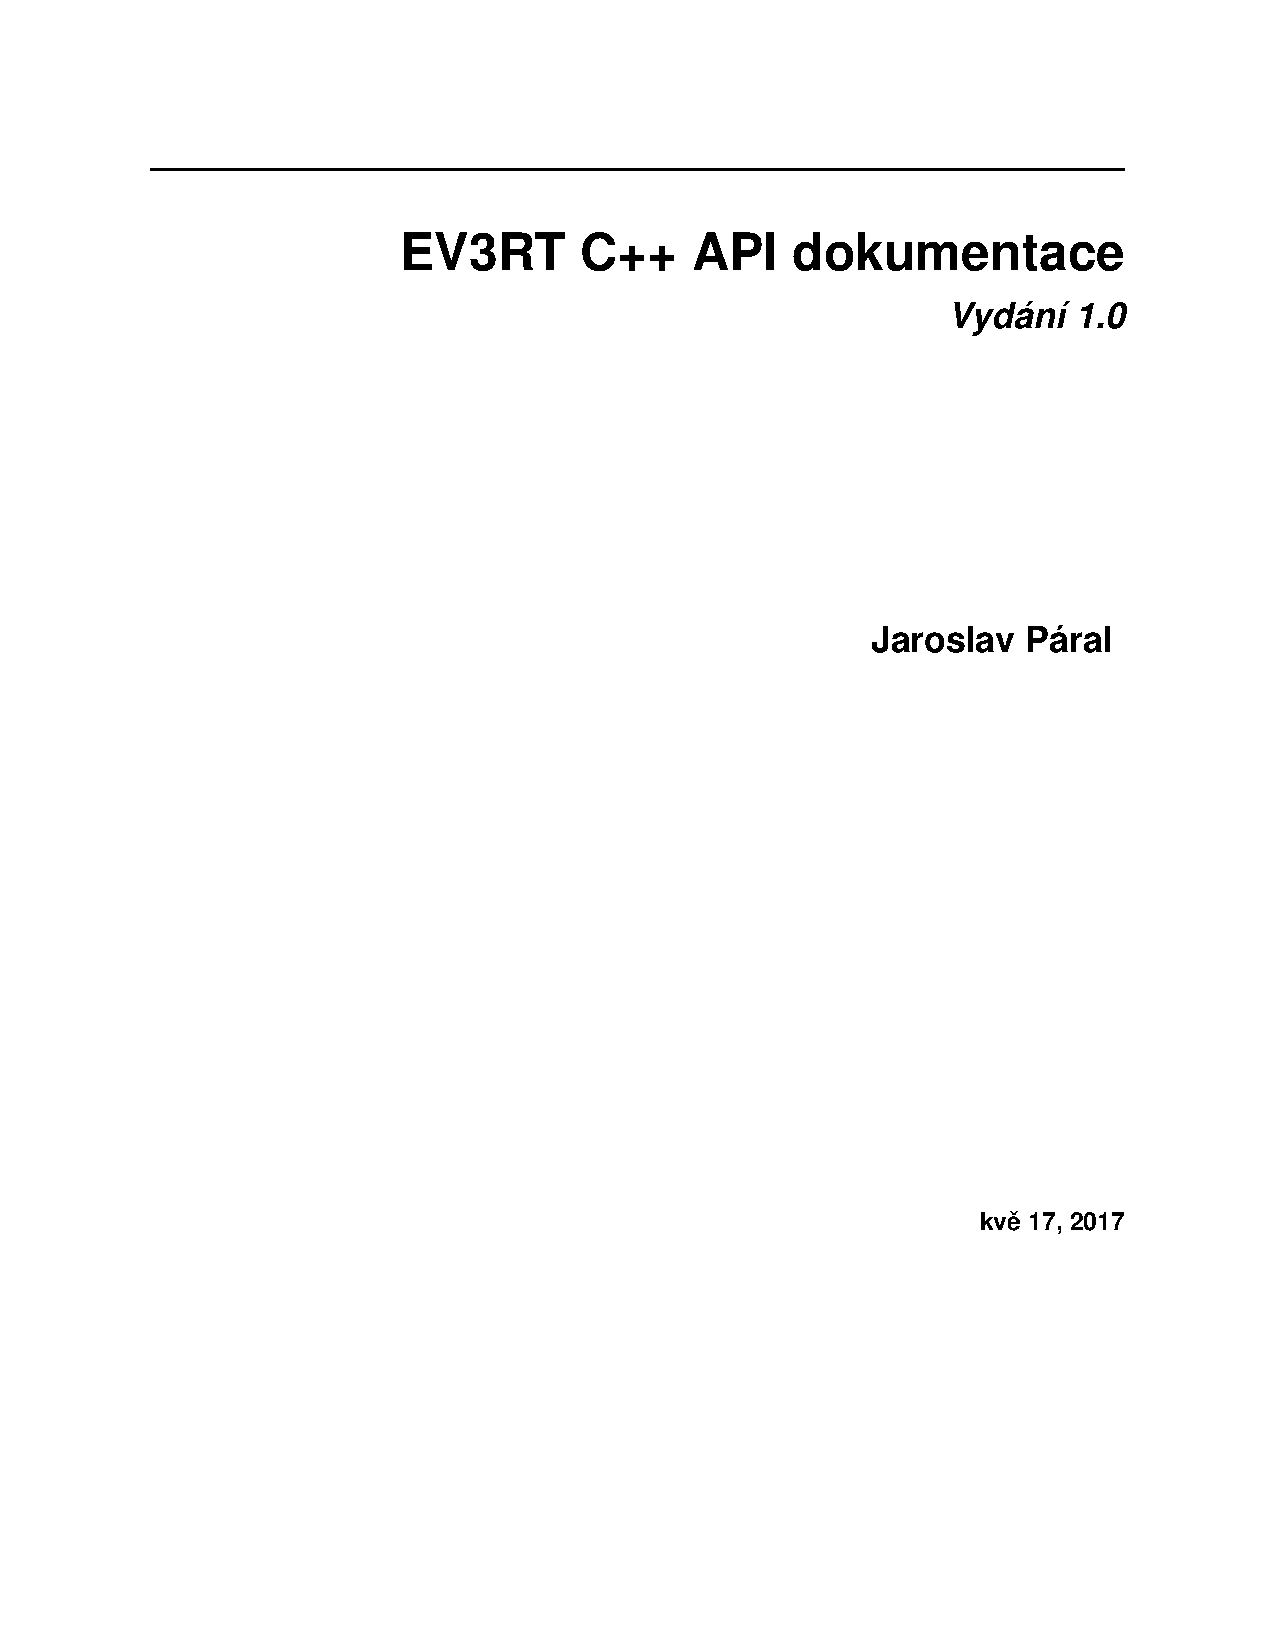
\includepdf[page=13]{ev3rt-cxx-api-doc.pdf}
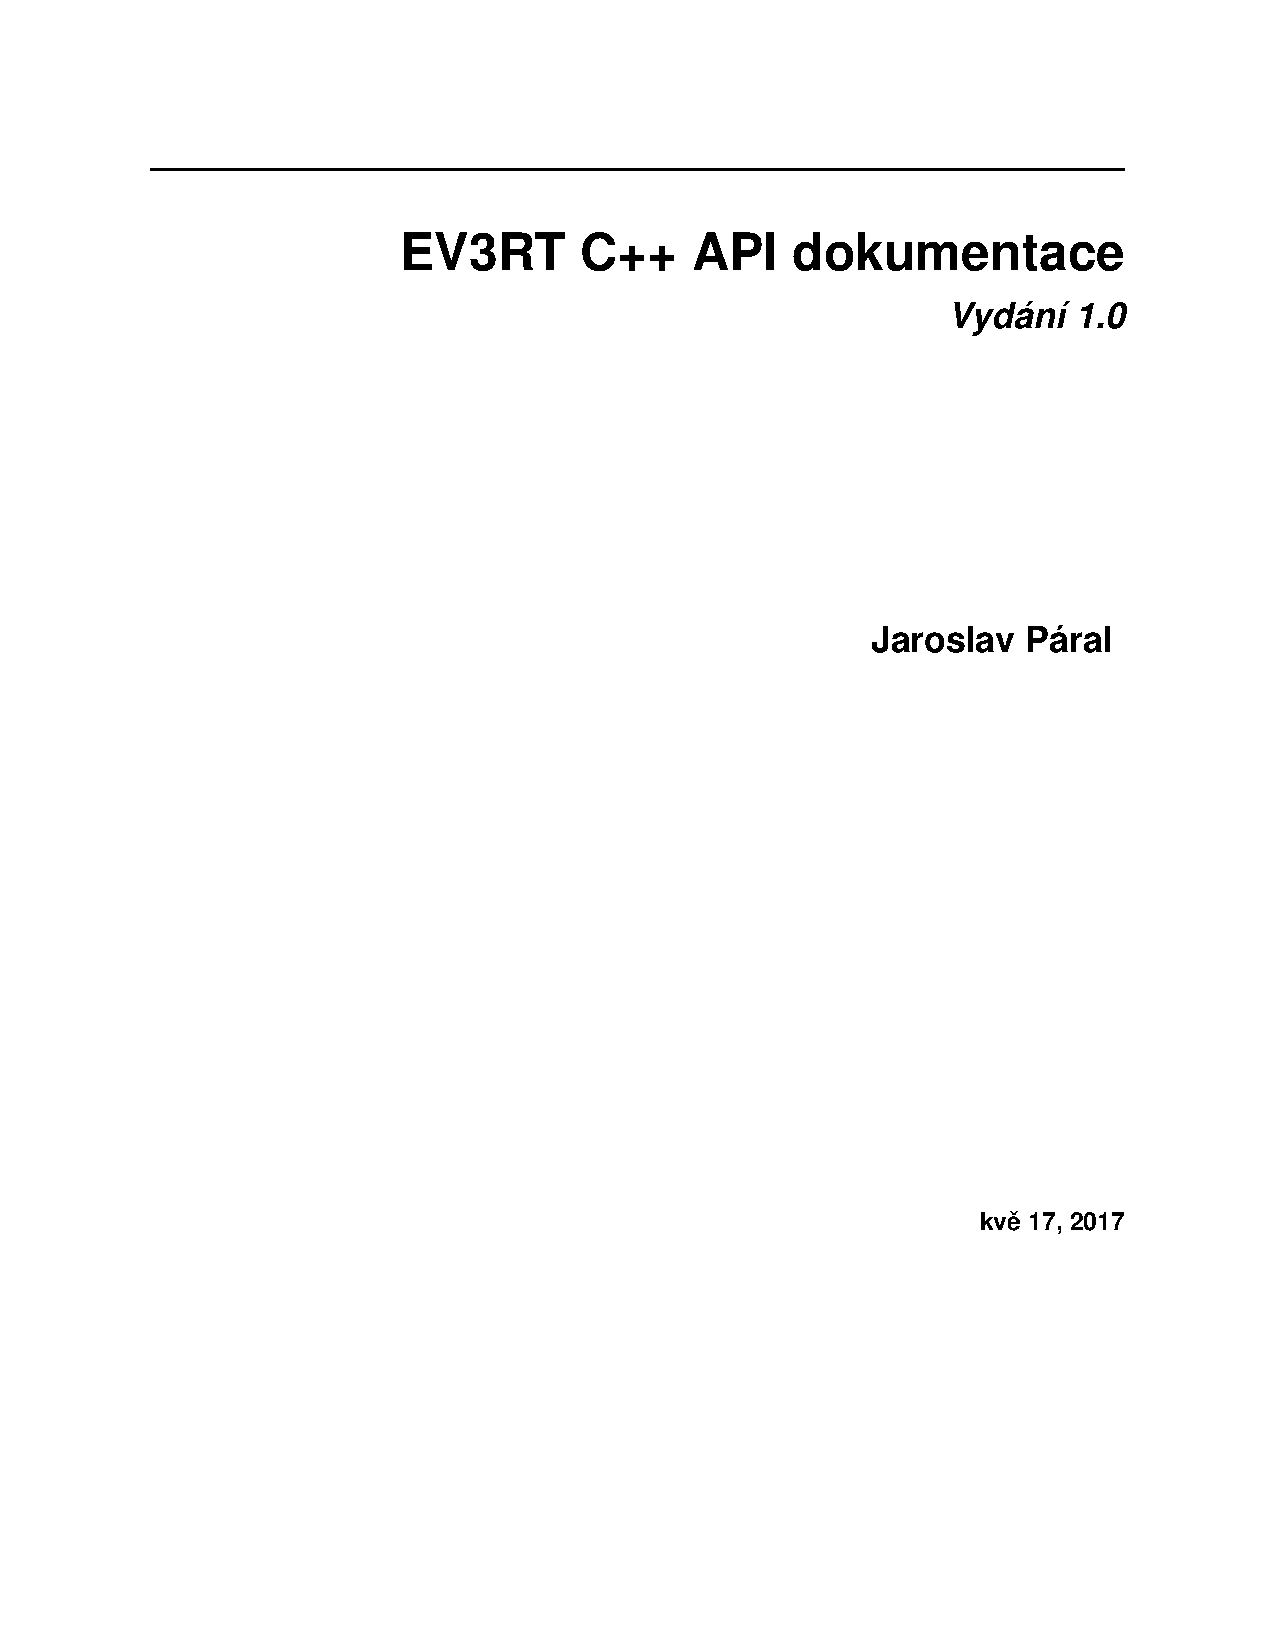
\includepdf[page=14]{ev3rt-cxx-api-doc.pdf}
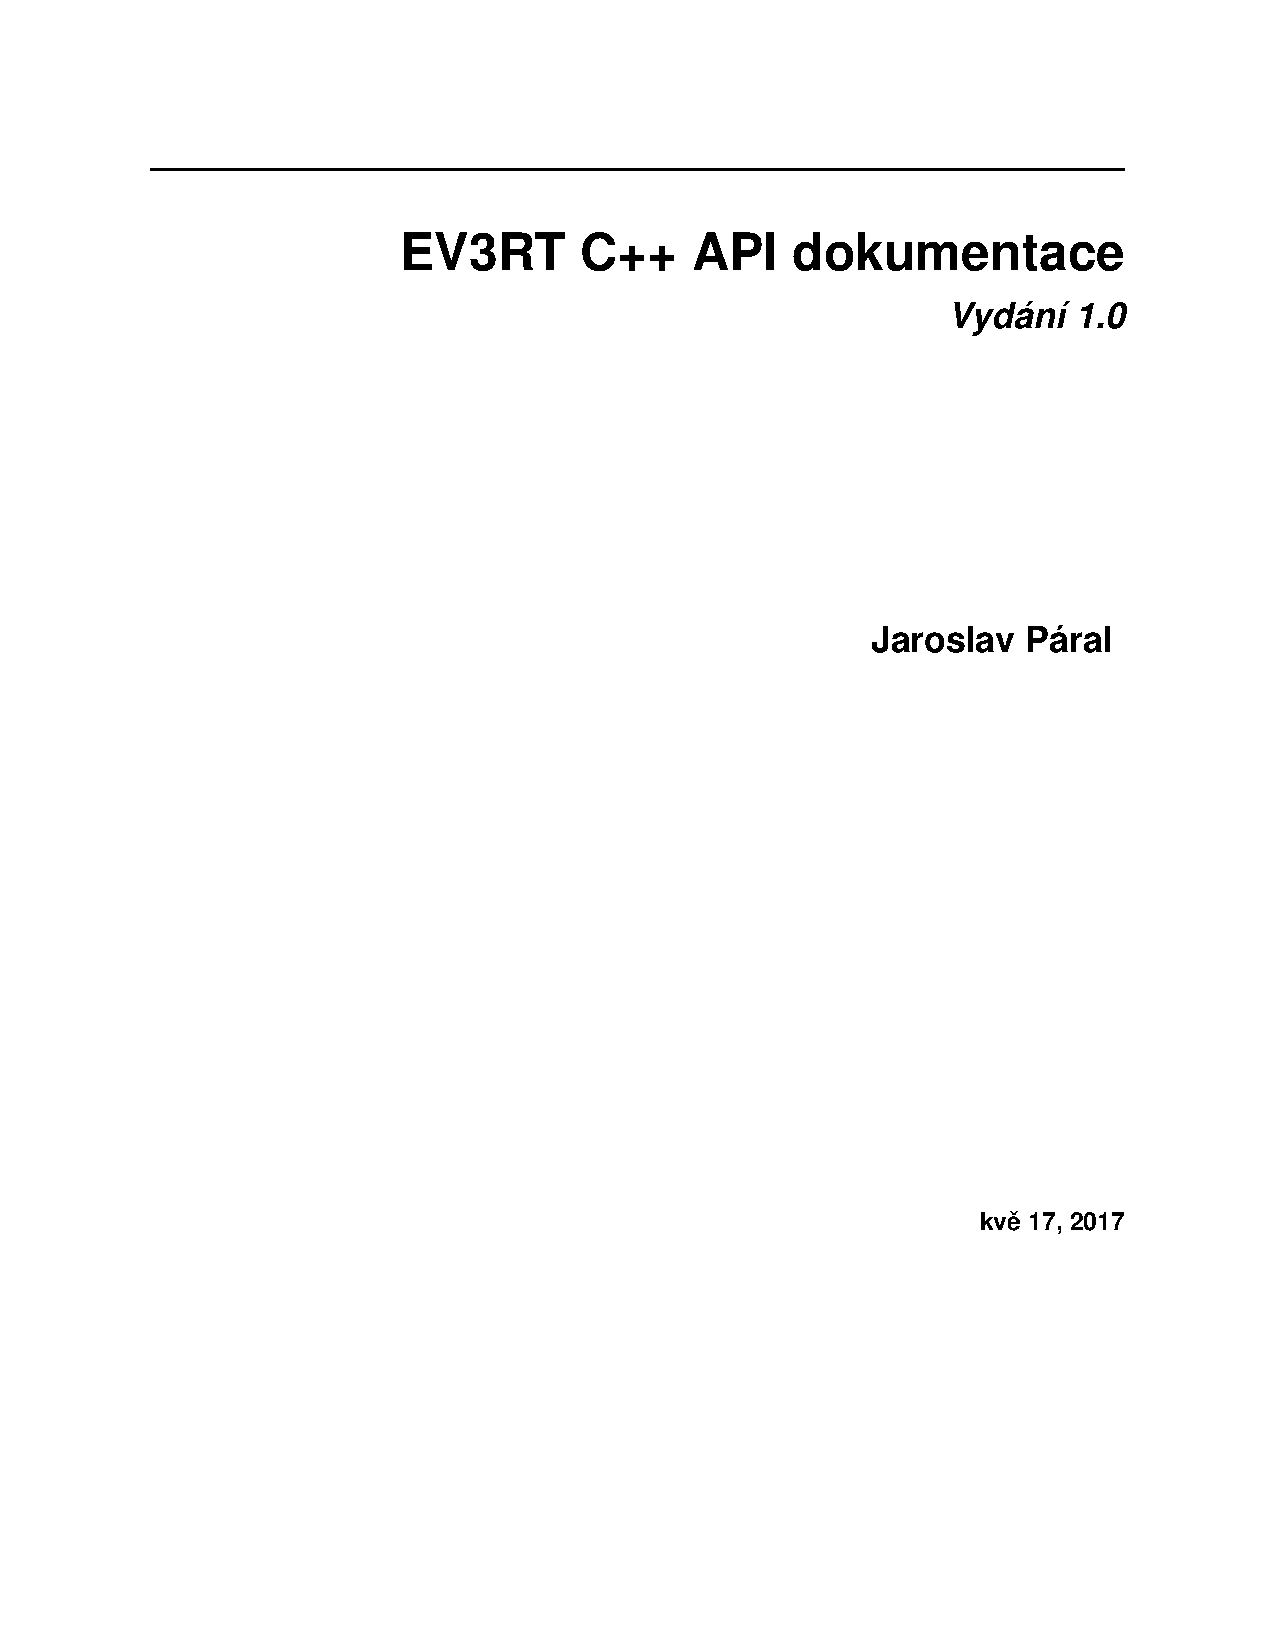
\includepdf[page=15]{ev3rt-cxx-api-doc.pdf}
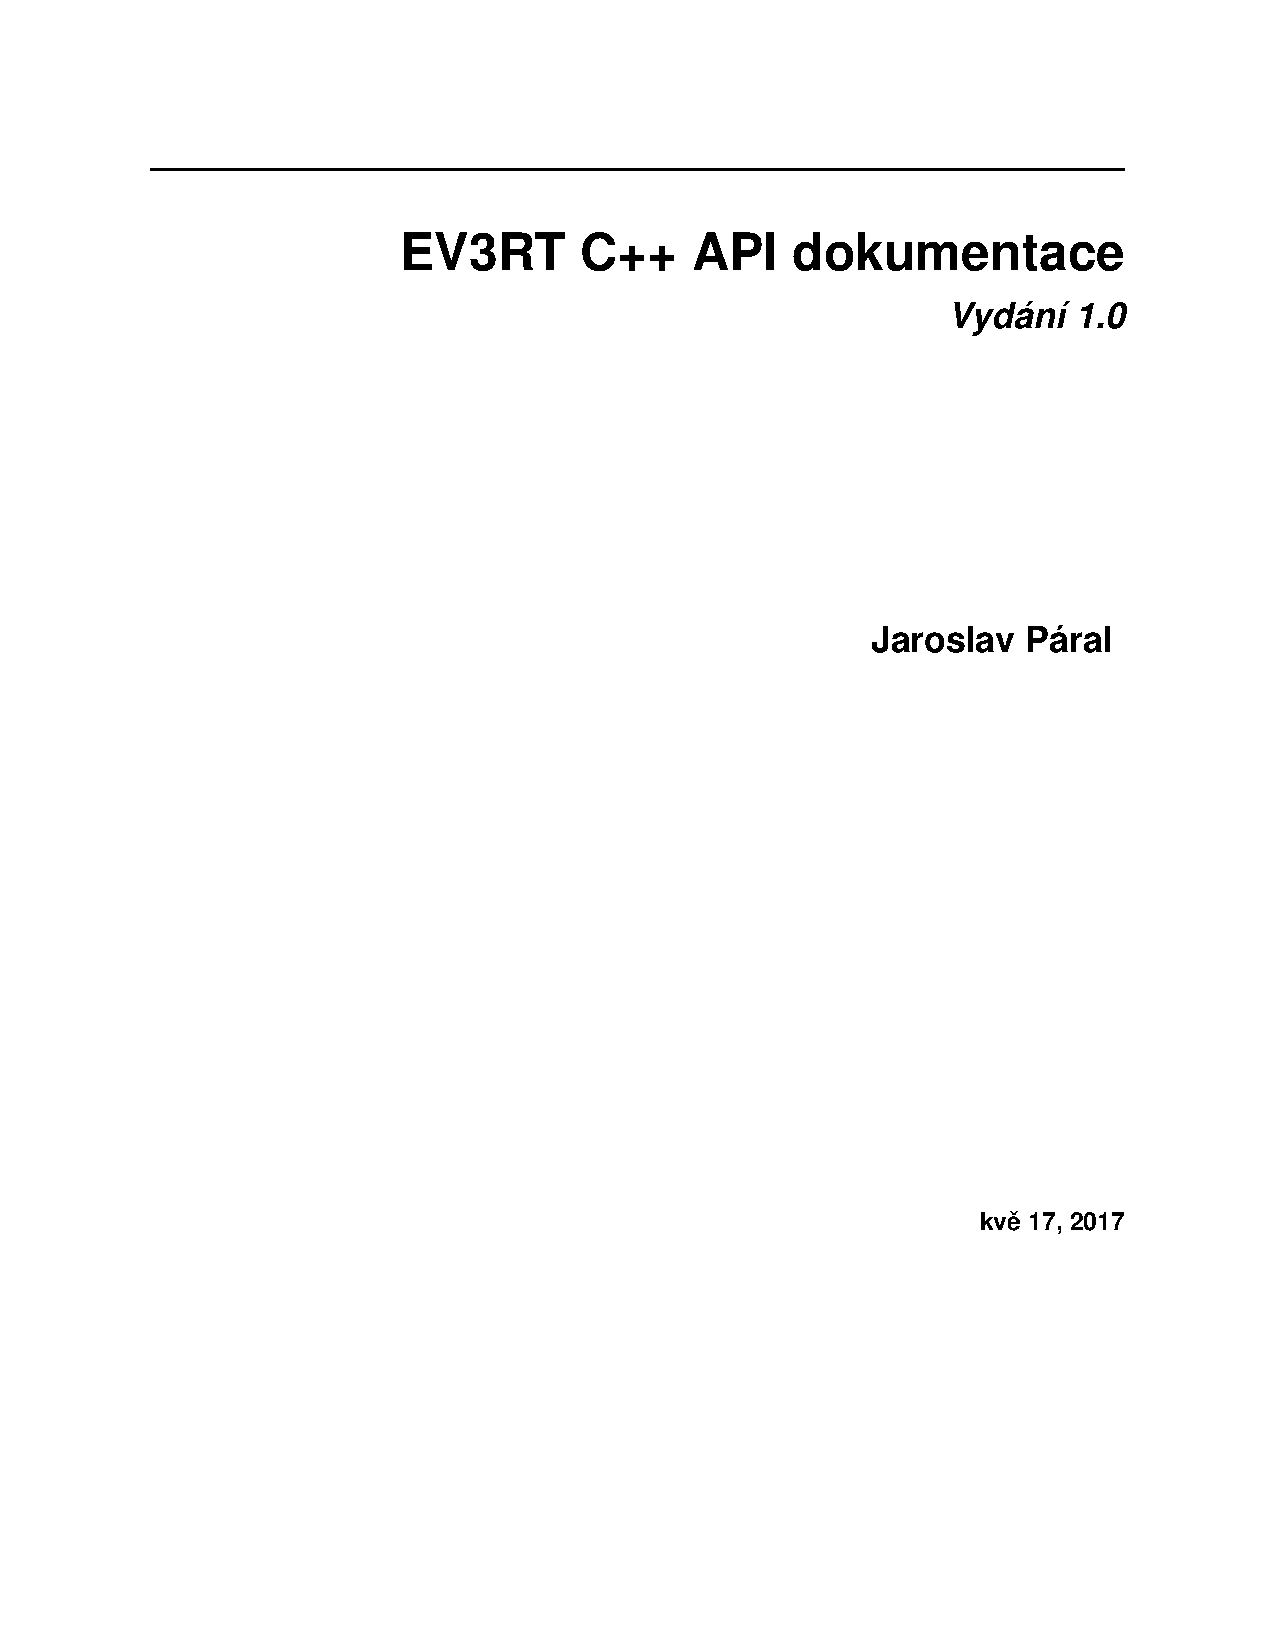
\includepdf[page=16]{ev3rt-cxx-api-doc.pdf}
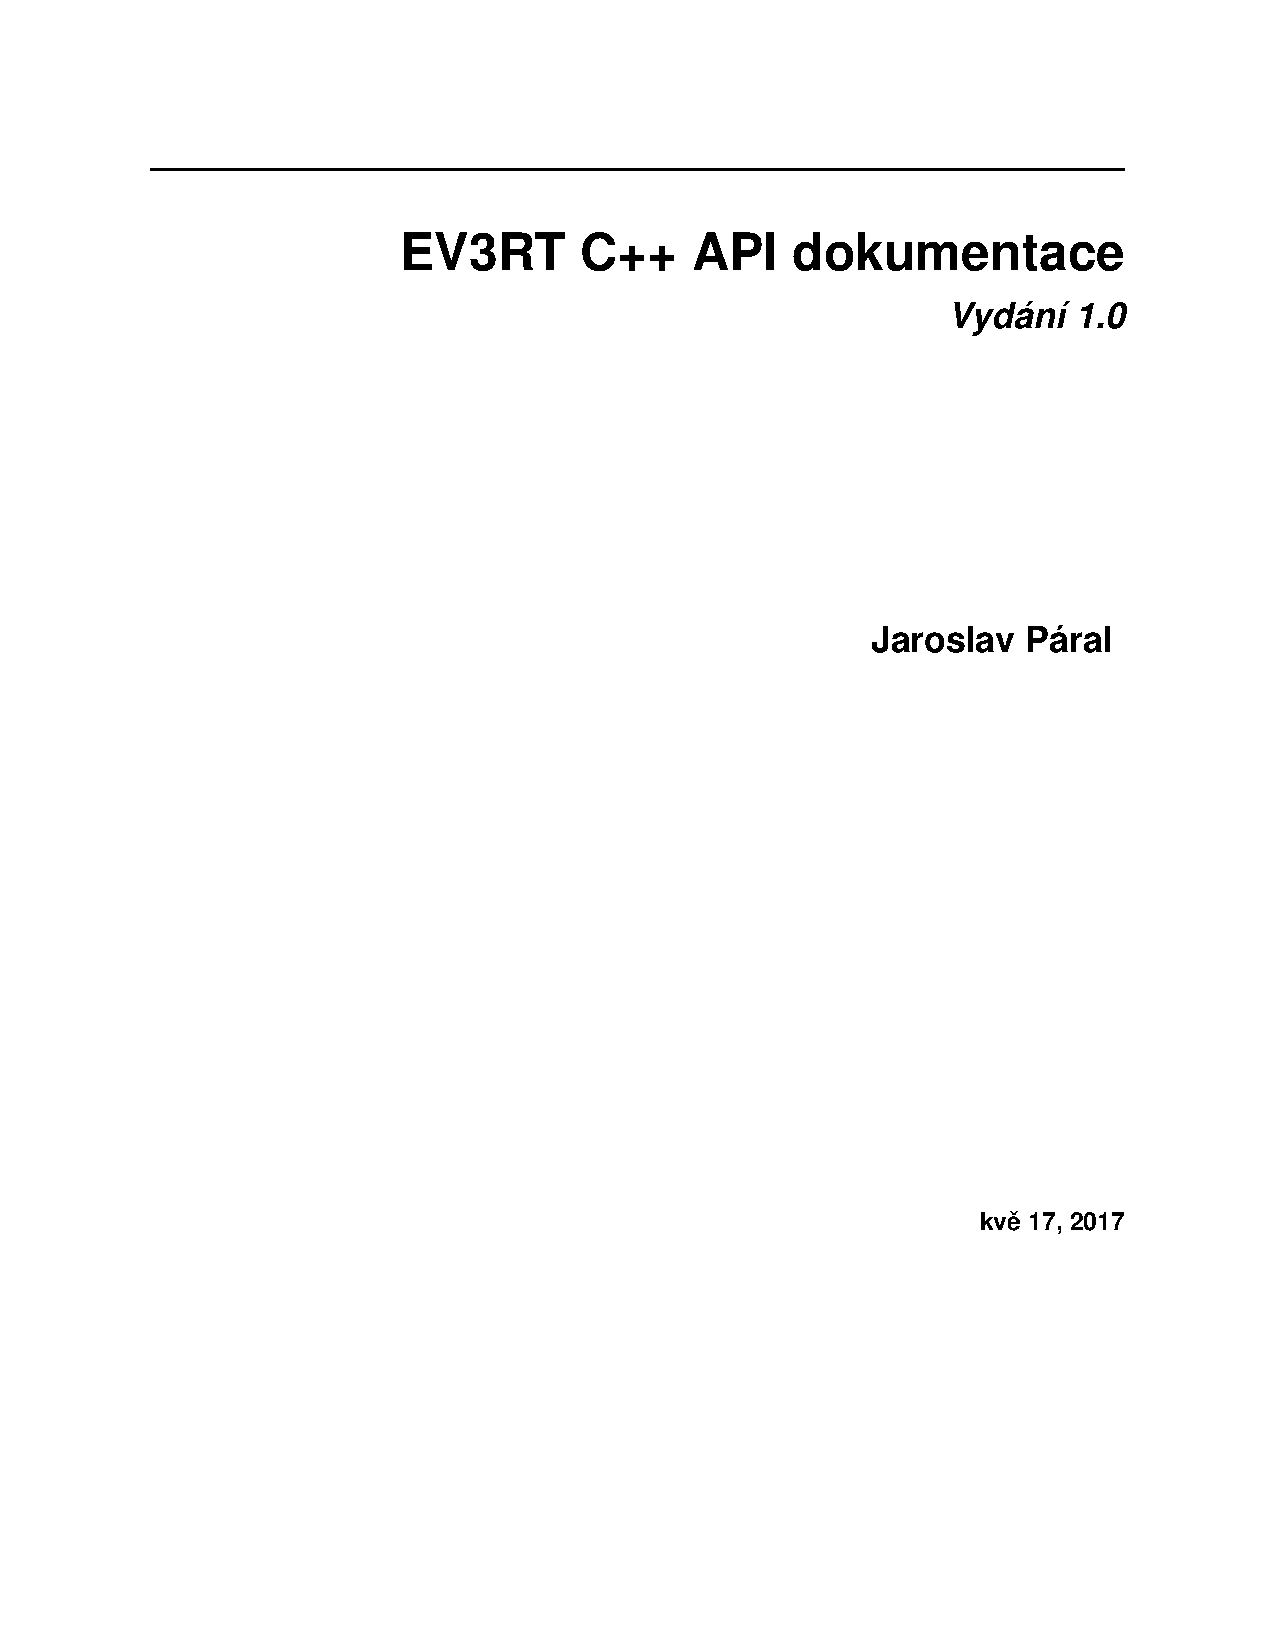
\includepdf[page=17]{ev3rt-cxx-api-doc.pdf}
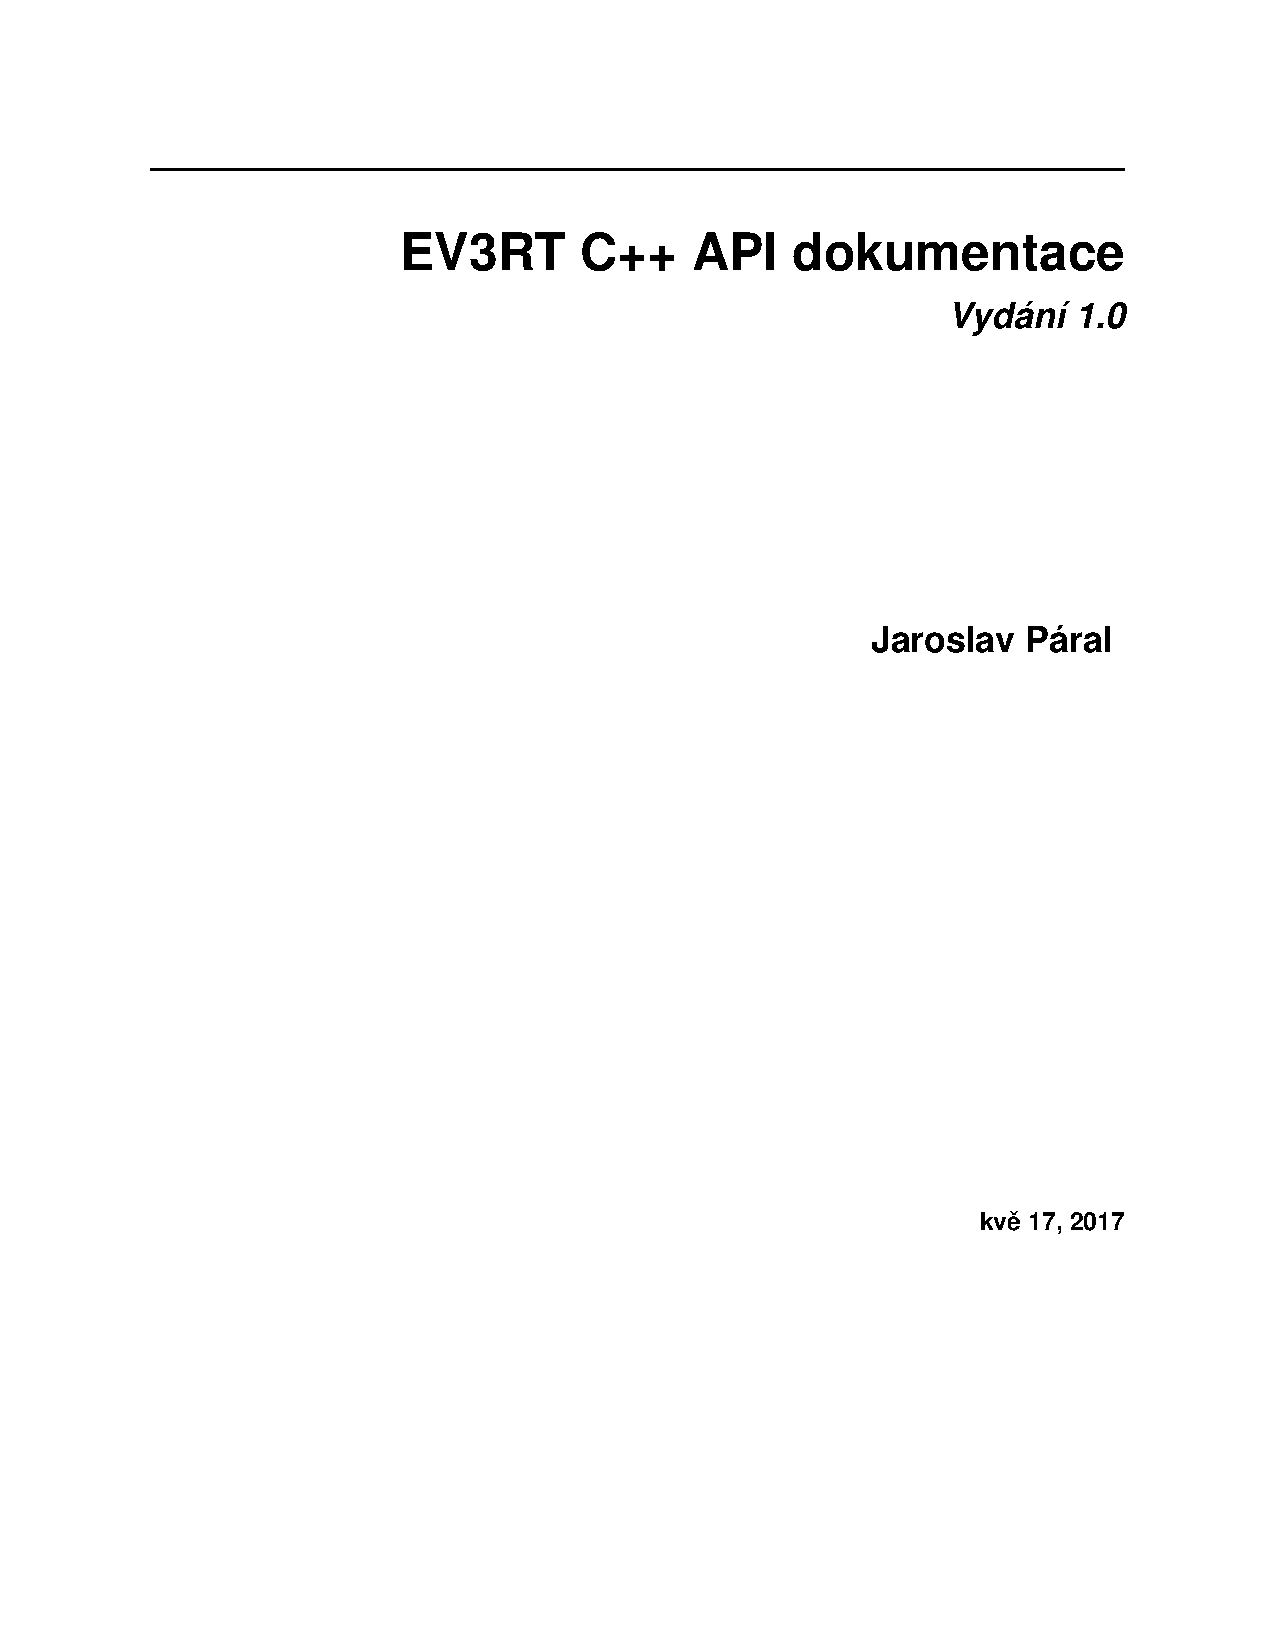
\includepdf[page=18]{ev3rt-cxx-api-doc.pdf}
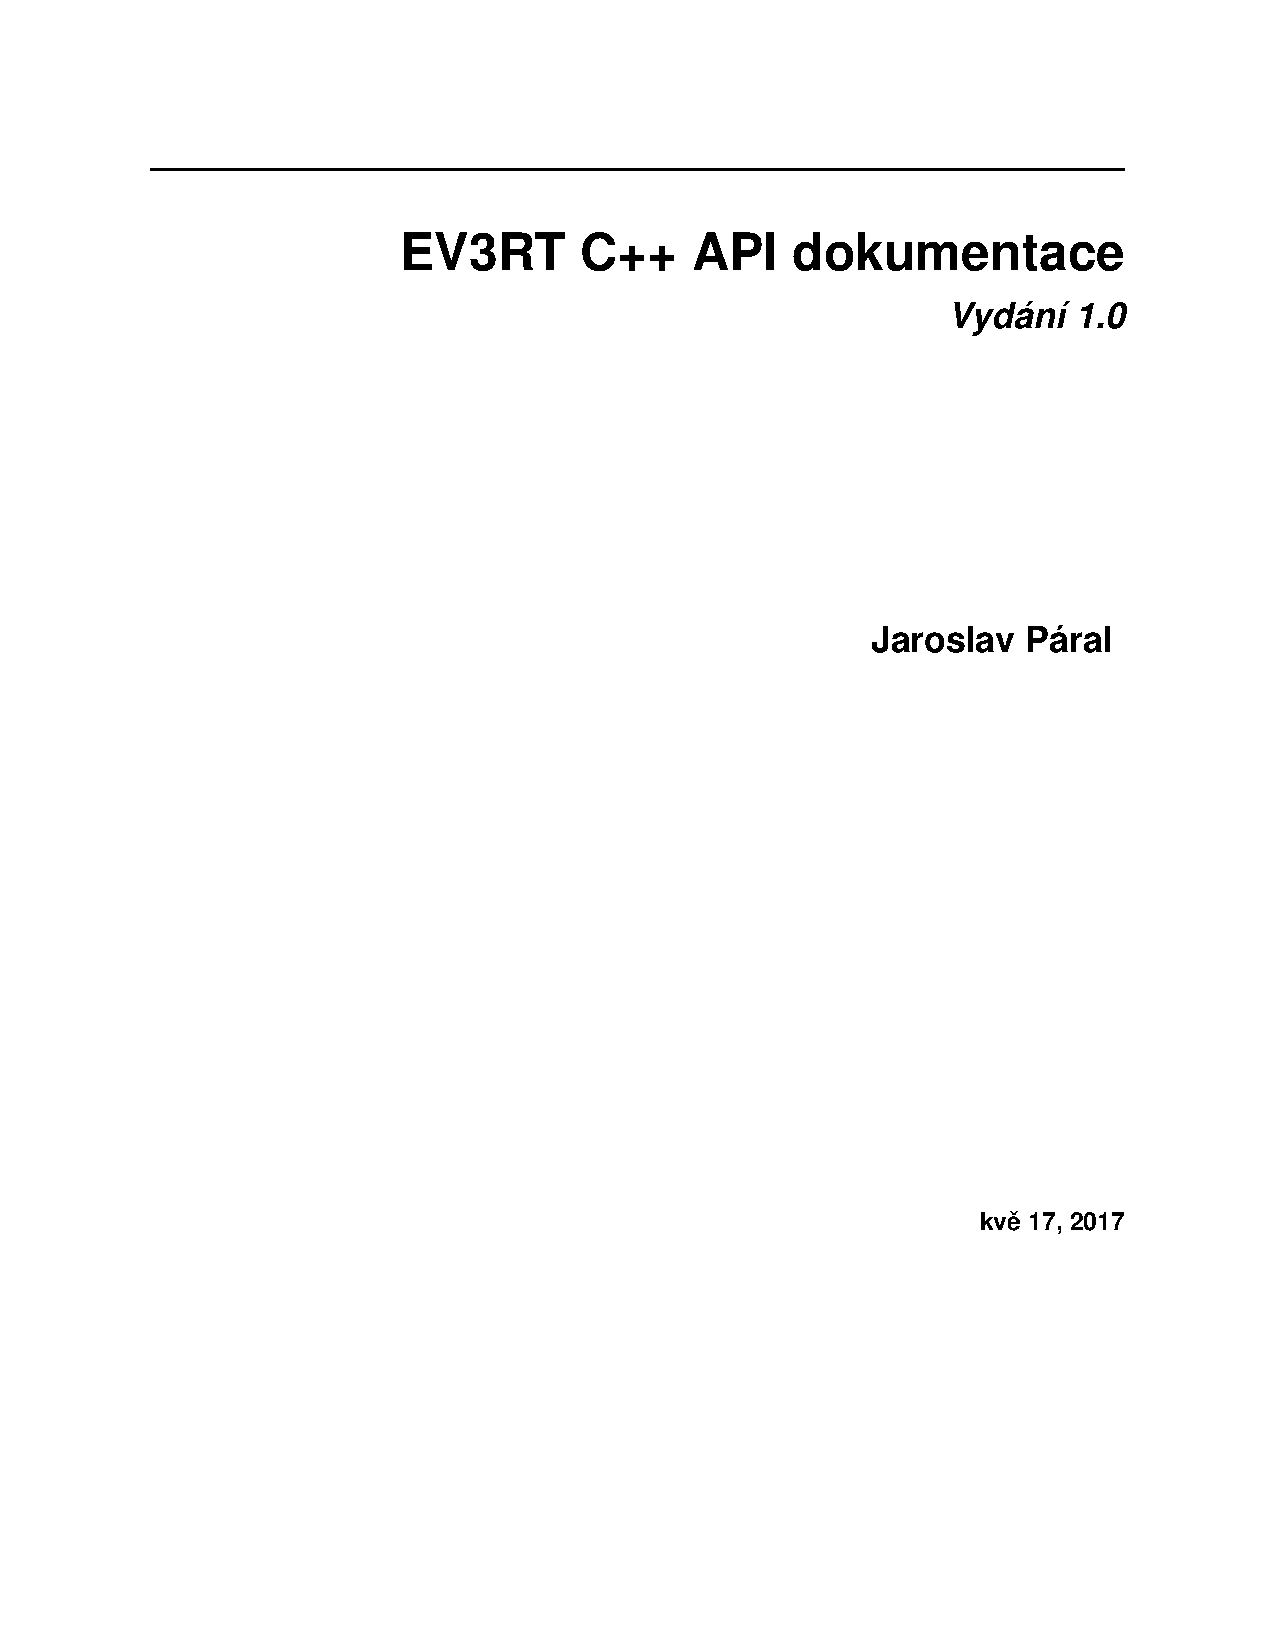
\includepdf[page=19]{ev3rt-cxx-api-doc.pdf}
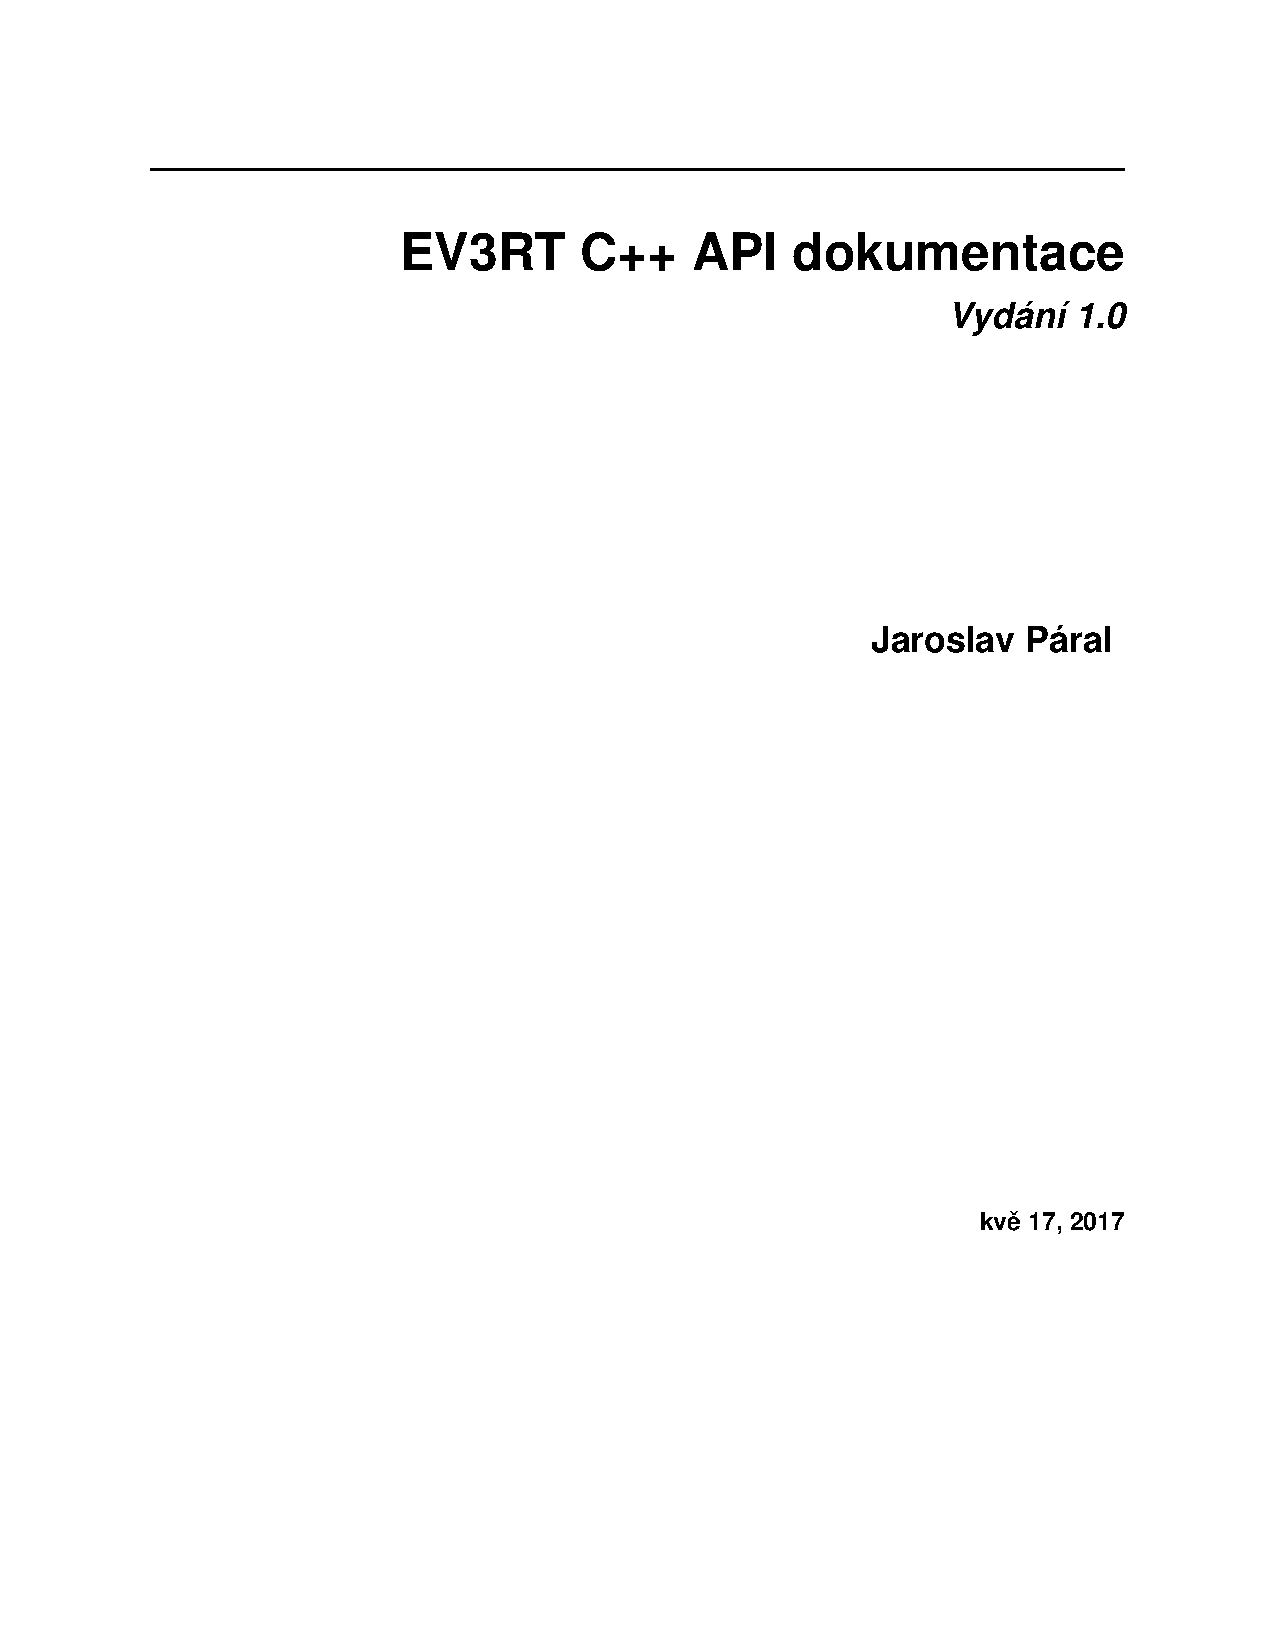
\includepdf[page=21]{ev3rt-cxx-api-doc.pdf}
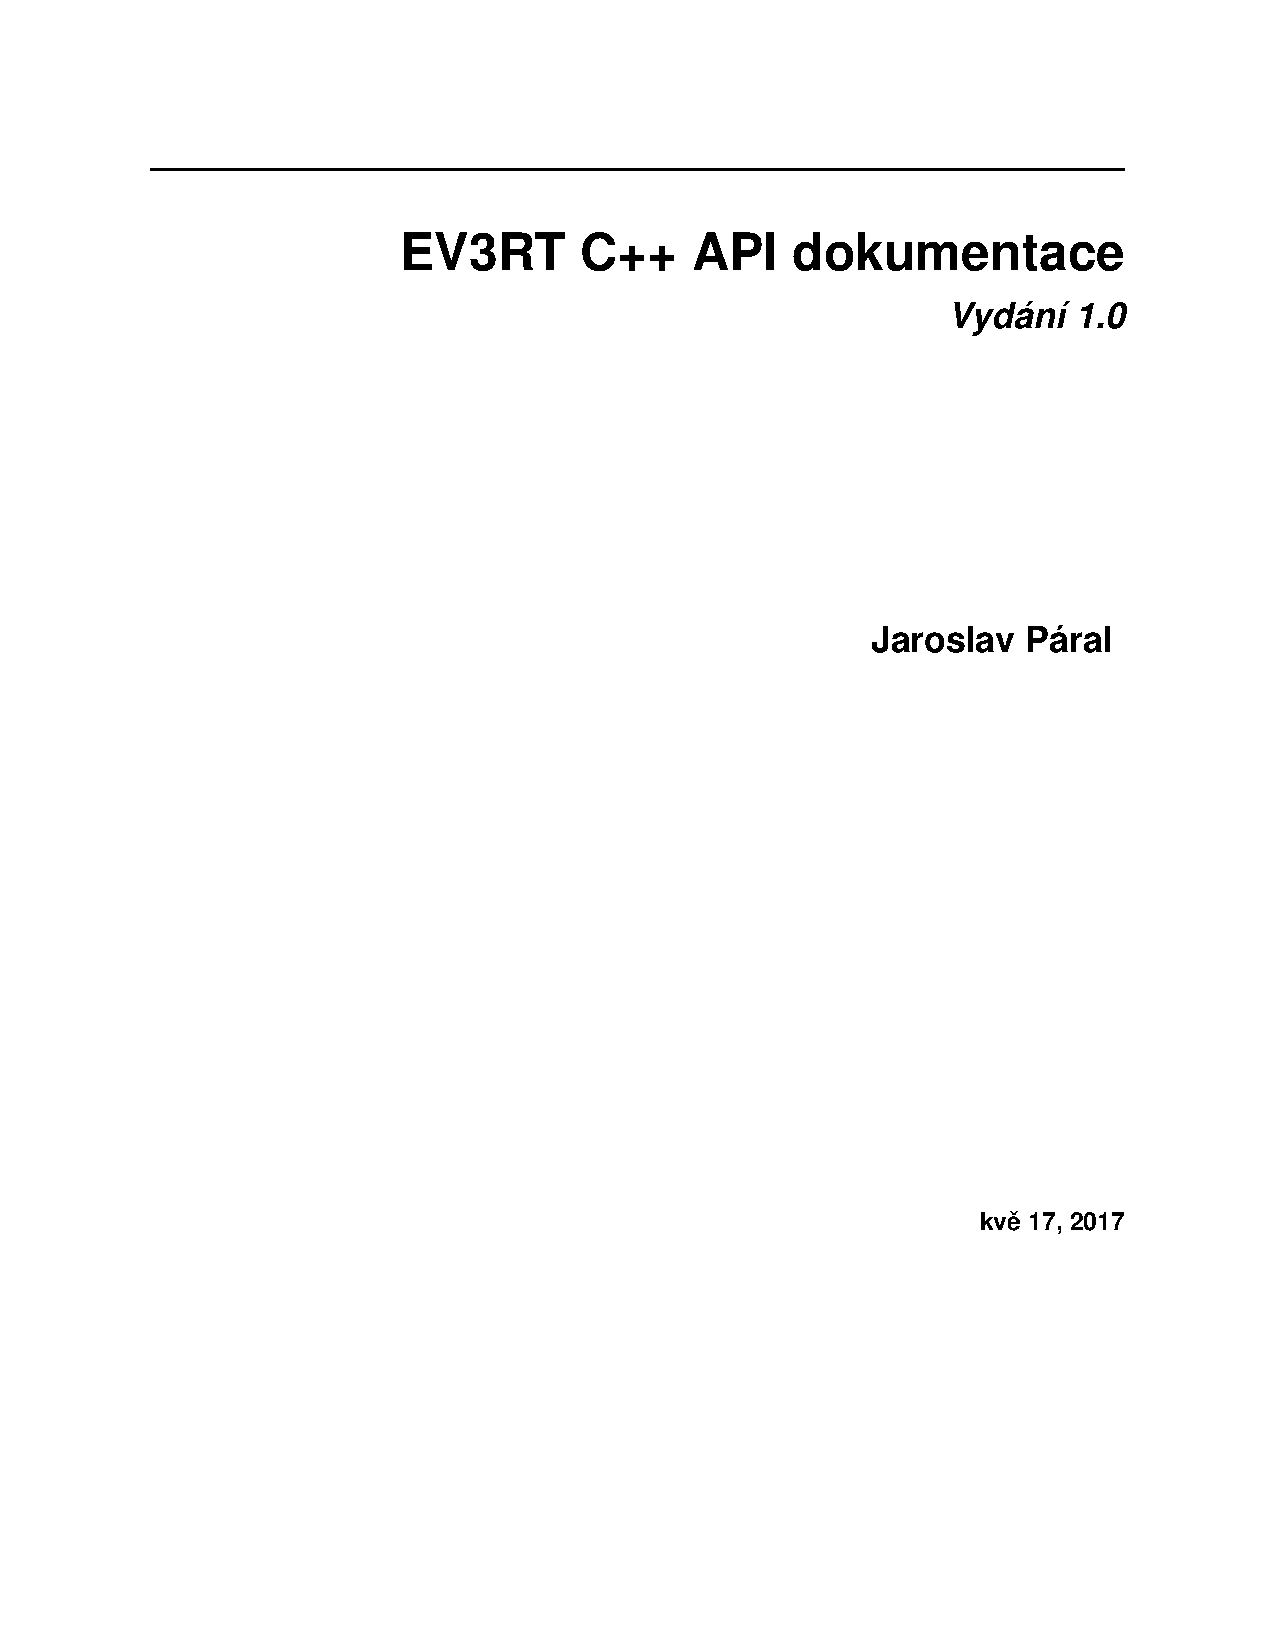
\includepdf[page=22]{ev3rt-cxx-api-doc.pdf}
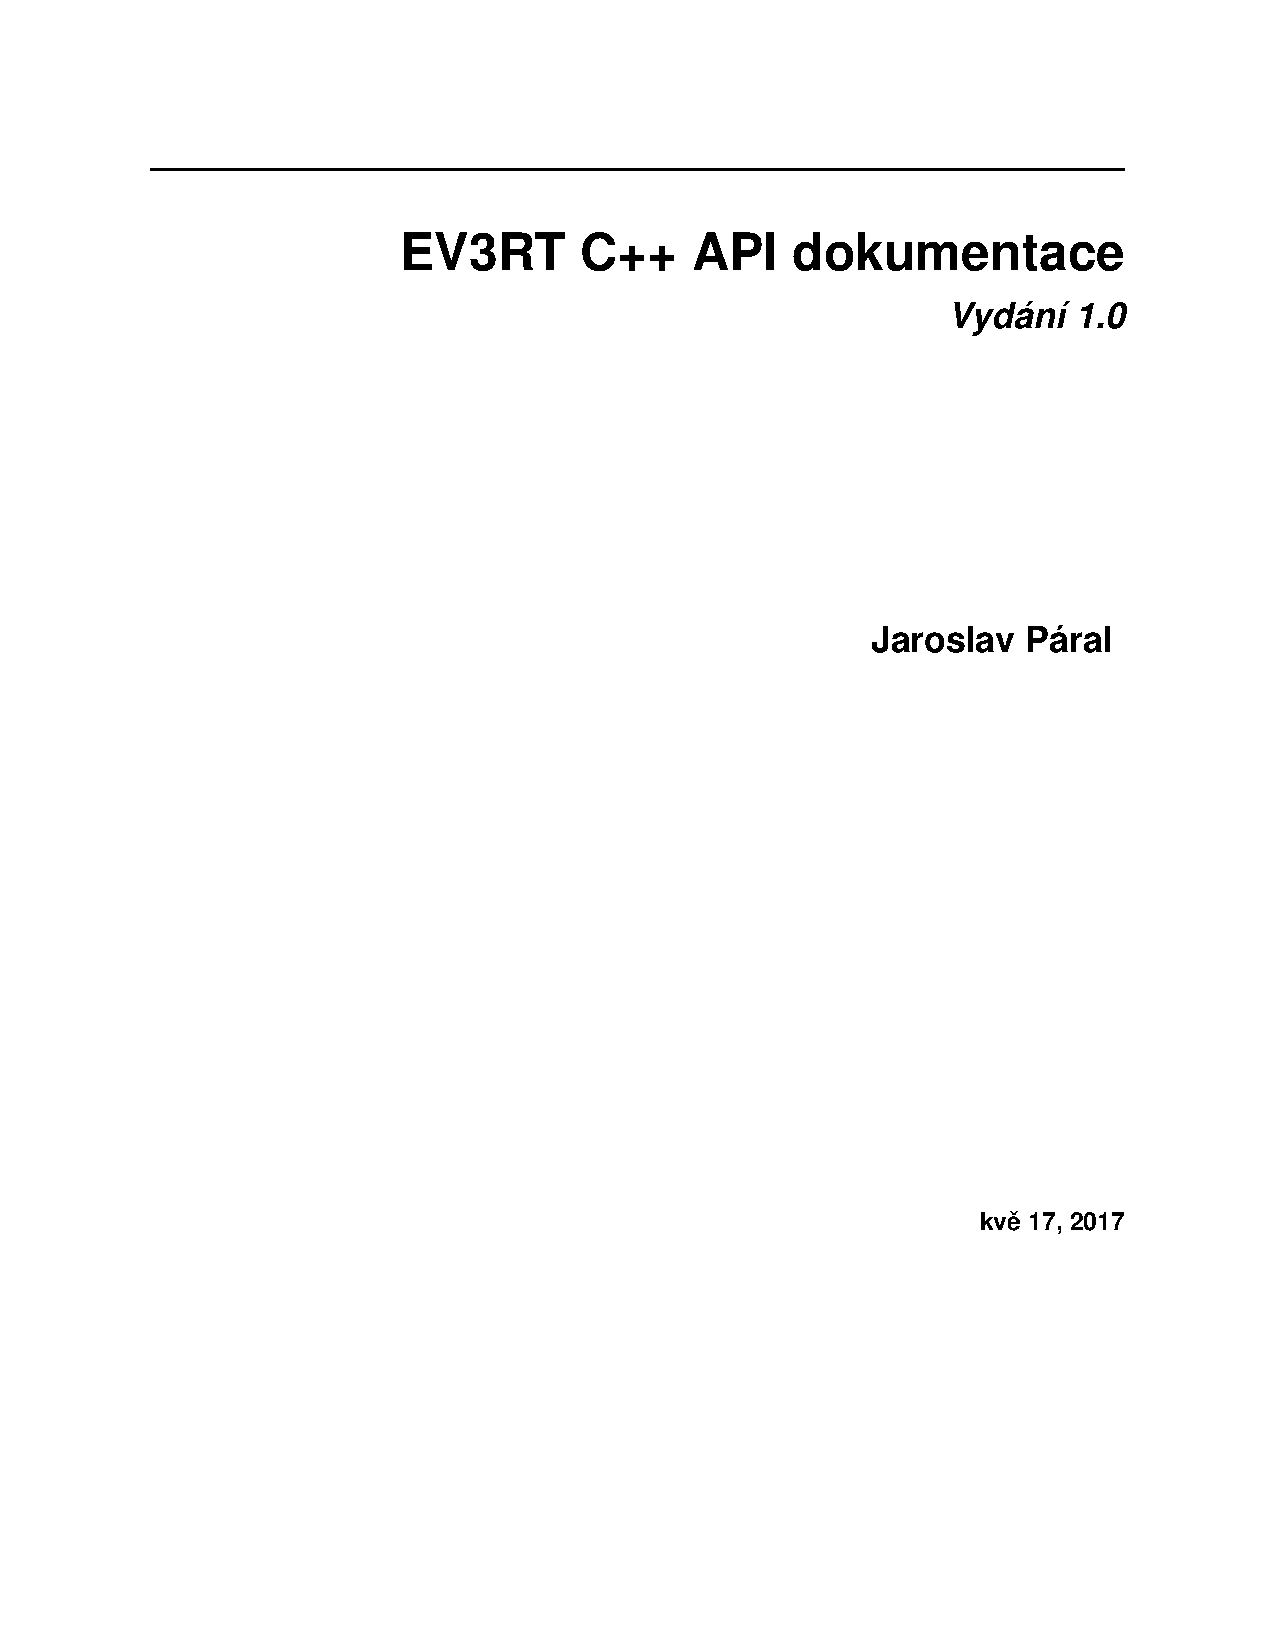
\includepdf[page=23]{ev3rt-cxx-api-doc.pdf}
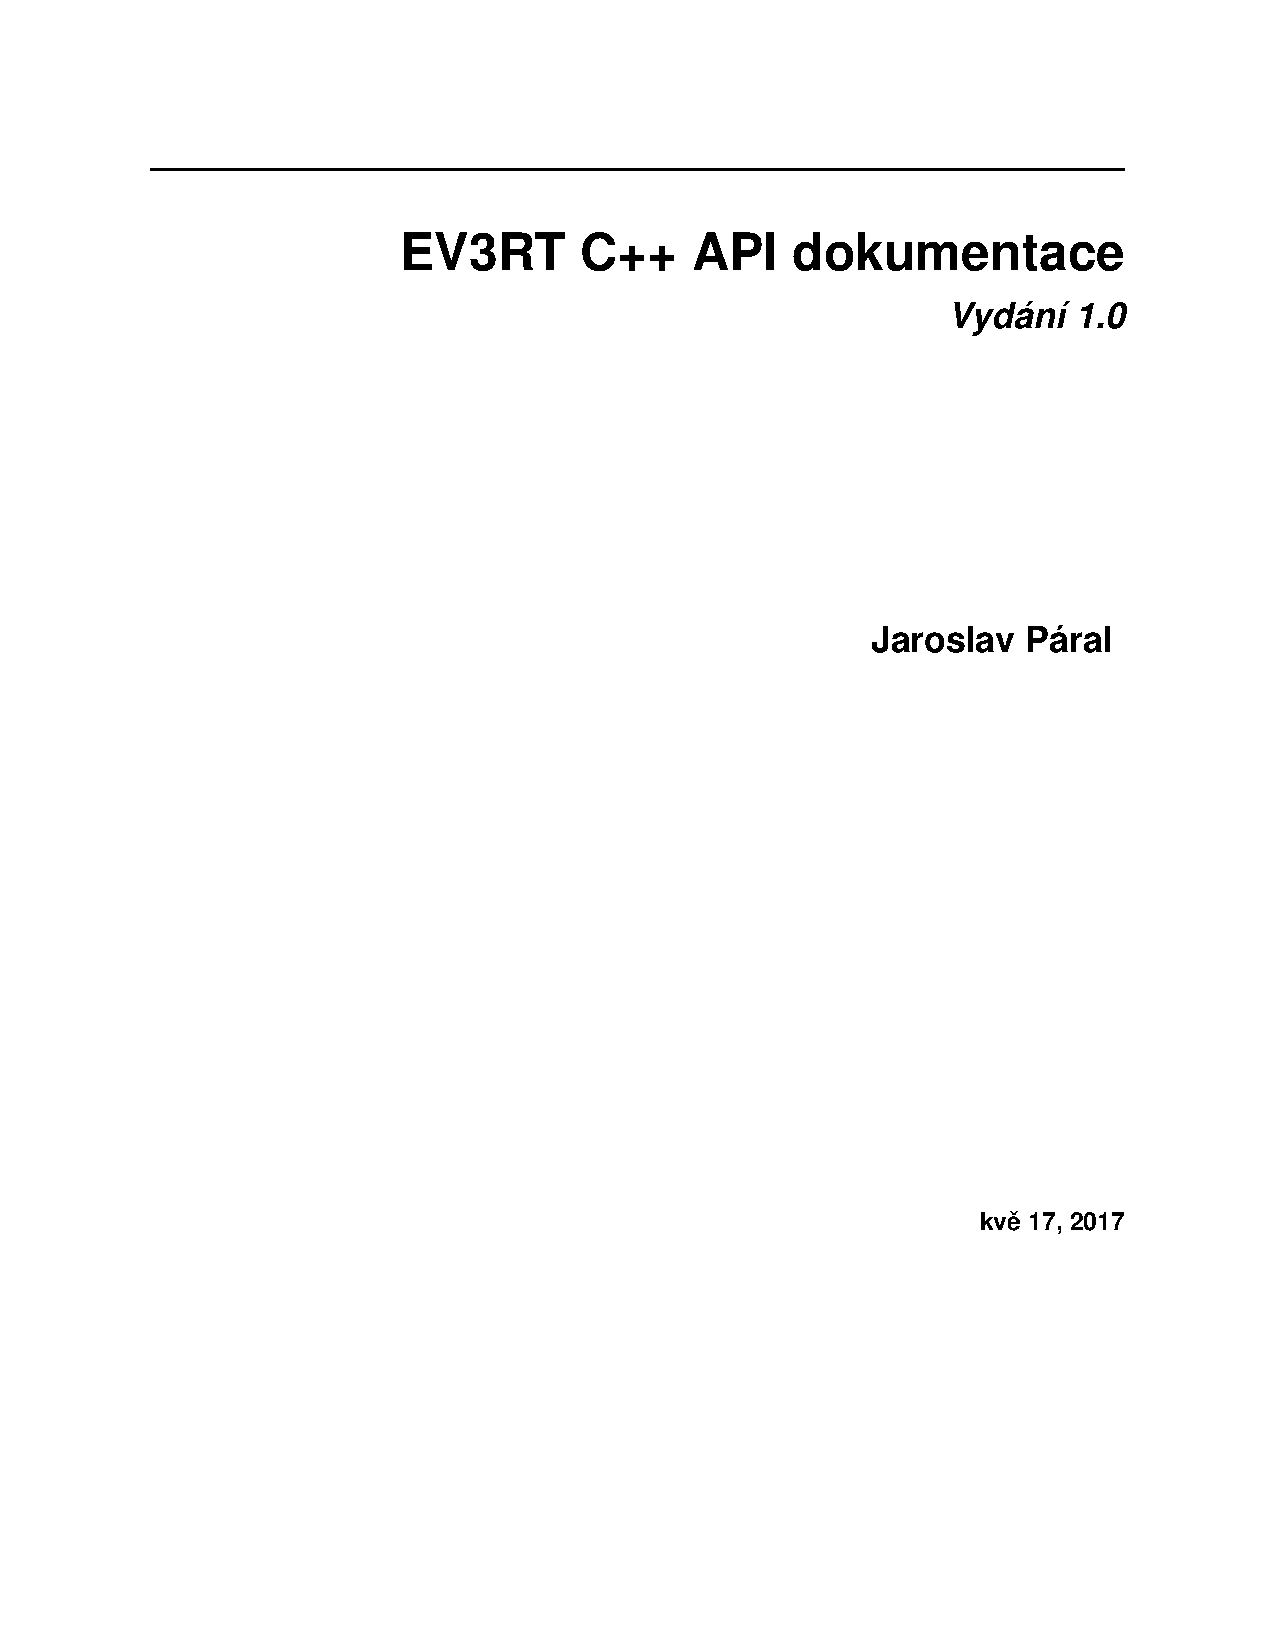
\includepdf[page=24]{ev3rt-cxx-api-doc.pdf}
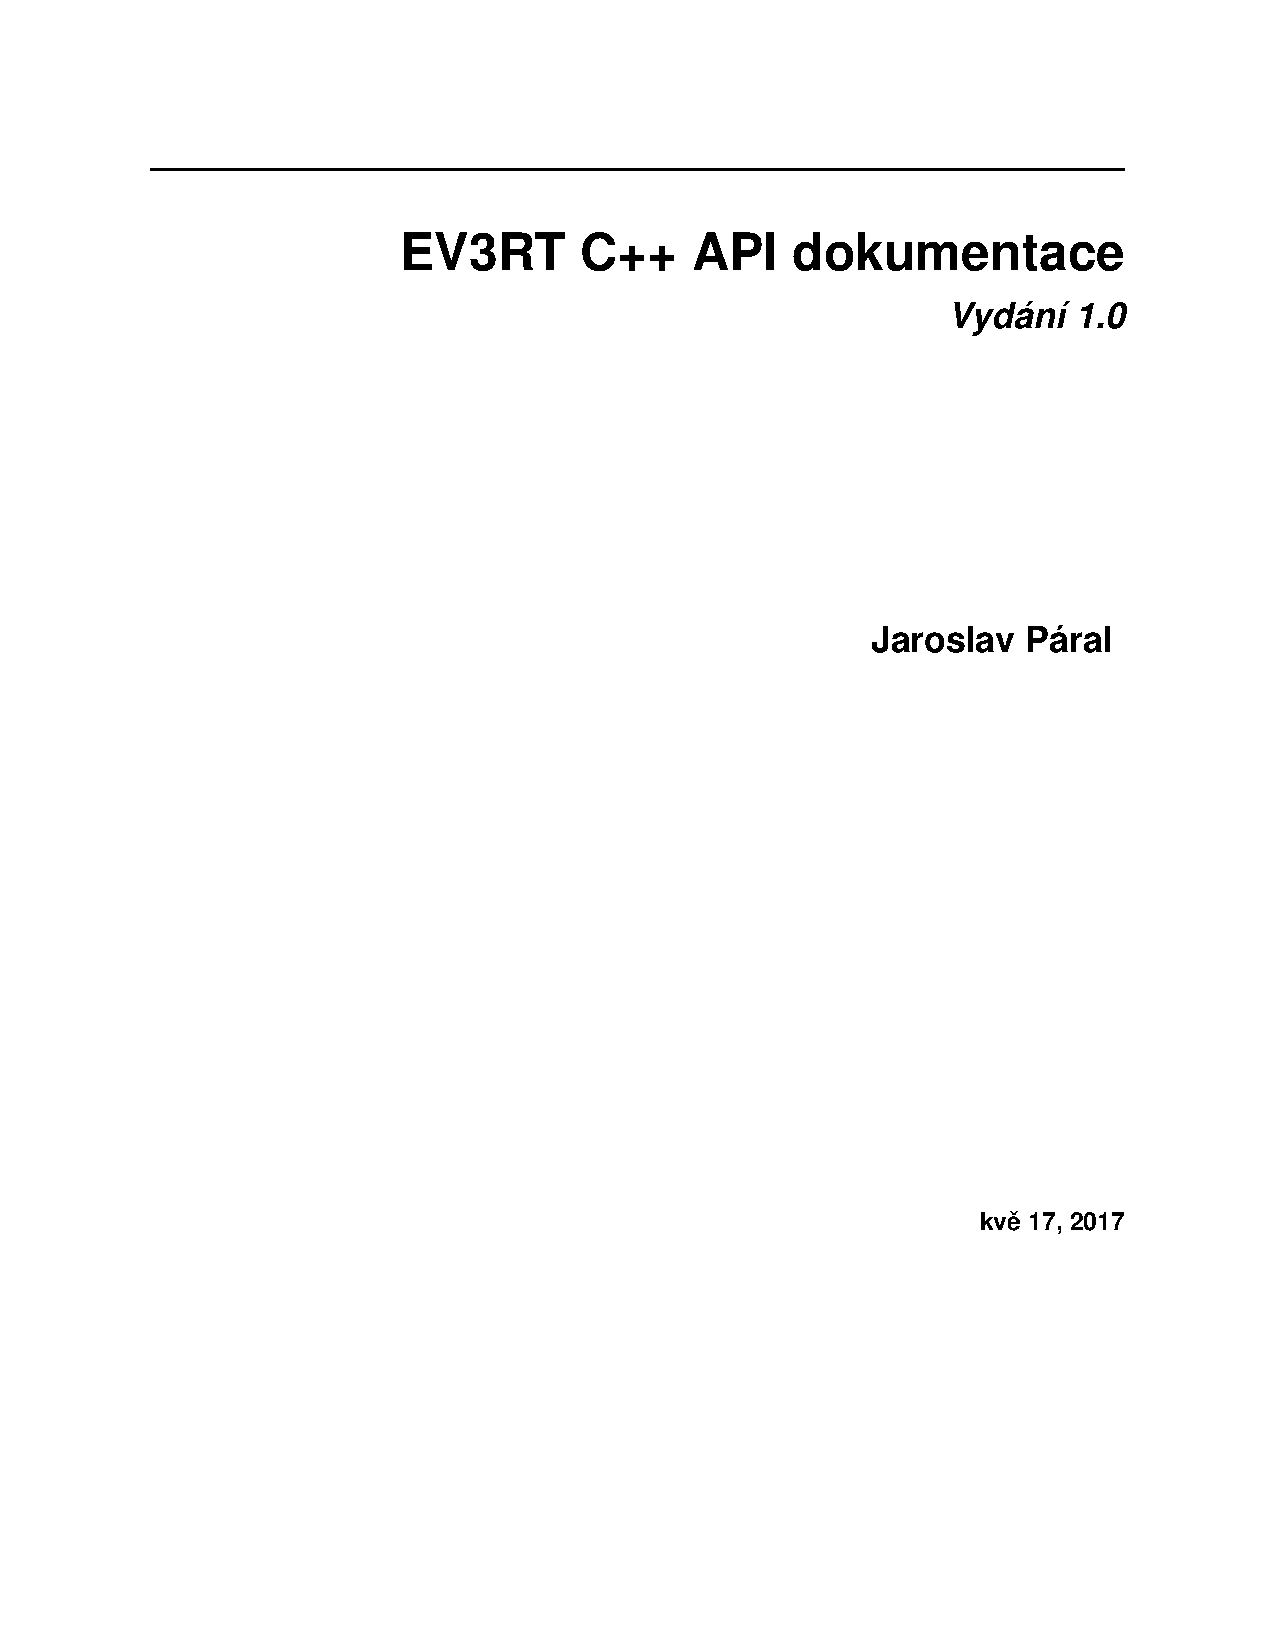
\includepdf[page=25]{ev3rt-cxx-api-doc.pdf}
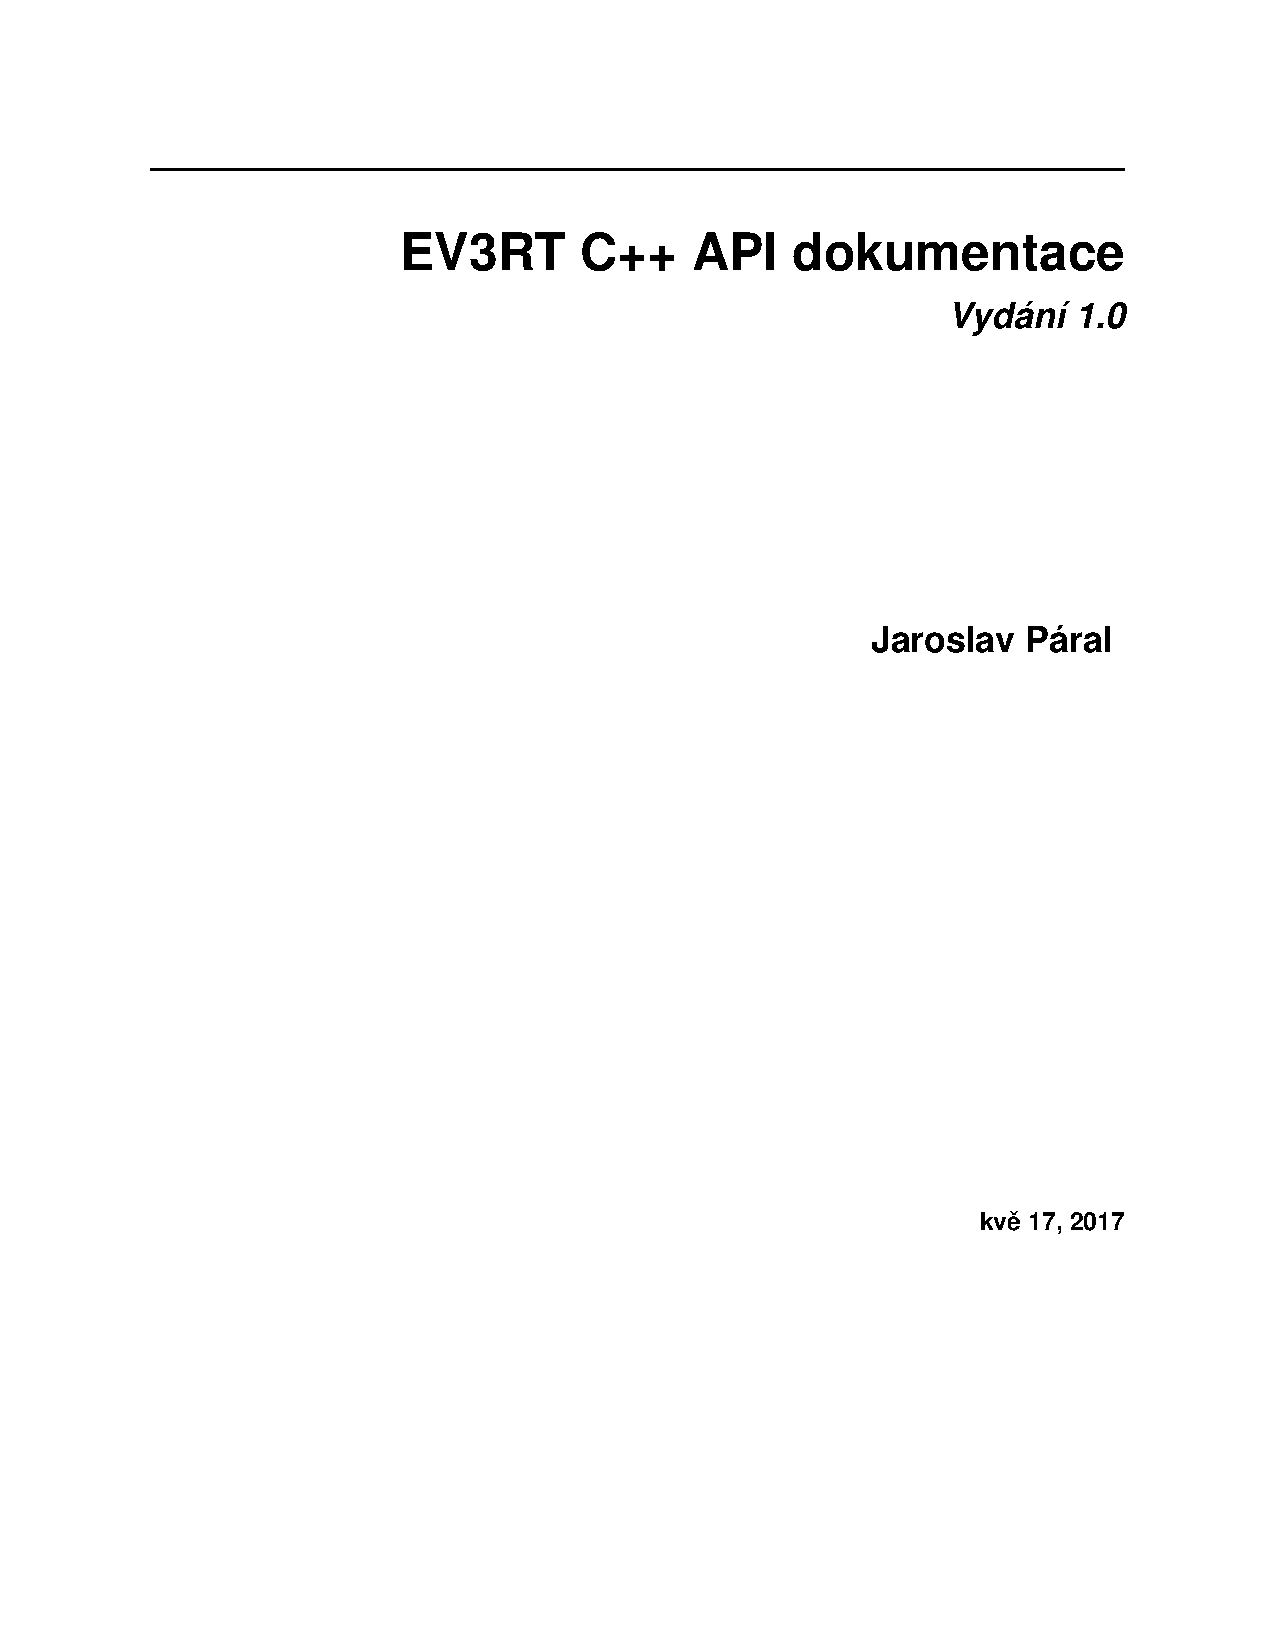
\includepdf[page=26]{ev3rt-cxx-api-doc.pdf}